\section{Sobre esta guía}\index{Sobre la guía}

La siguiente guía tiene como objetivo presentar de manera sistemática los contenidos teórico práctico de la asignatura \textbf{Programación de aplicaciones web} en base al plan de carrera del Instituto Tecnológico Benito Juárez en su rediseño del año 2016 para Desarrollo de Software.

\begin{center}
	Datos generales de la asignatura\\
		\begin{tabular}{ |c|c| } 
			\hline
			Nombre de la asignatura: & Programación Aplicaciones Web \\
			\hline
			Campo de formación: & Adaptación tecnológica e innovación \\ 
			\hline
			Unidad de organización curricular: & Formación técnica profesional \\
			\hline
			Número de período académico: & 4 \\
			\hline
			Número de horas de la asignatura: & 122 \\
			\hline
			Número de horas por cada componente: & 
			\begin{tabular}{c}
				Docencia: 60\\
				Prácticas de aprendizaje: 24 \\ 
				Aprendizaje autónomo: 38 \\
			\end{tabular} \\
			\hline
			Docente: & Freddy Heredia: \textbf{\texttt{fheredia@yavirac.edu.ec}}\\
			\hline
		\end{tabular}
\end{center}

\chapter{Conceptos generales}

\section{El origen} \index{El origen}

\cite{sl}Aunque los inicios de Internet se remontan a los años setenta, no ha sido hasta los años noventa cuando, gracias a la Web, se ha extendido su uso por todo el mundo. En pocos años la Web ha evolucionado enormemente: se ha pasado de páginas sencillas, con pocas imágenes y contenidos estáticos a páginas complejas con contenidos dinámicos que provienen de bases de datos, lo que permite la creación de "aplicaciones web".

\cite{sl}Internet y la Web han incluido enormemente tanto en el mundo de la informática
como en la sociedad en general. Si nos centramos en la Web, en poco menos de 10
años ha transformado los sistemas informáticos: ha roto las barreras físicas (debido a
la distancia), económicas y lógicas (debido al empleo de distintos sistemas operativos,
protocolos, etc.) y ha abierto todo un abanico de nuevas posibilidades. Una de las áreas
que más expansión está teniendo en la Web en los últimos años son las aplicaciones
web.

\cite{sl}Las aplicaciones web permiten la generación automática de contenido, la creación
de páginas personalizadas según el perfil del usuario o el desarrollo del comercio electrónico. Además, una aplicación web permite interactuar con los sistemas informáticos de gestión de una empresa, como puede ser gestión de clientes, contabilidad o
inventario, a través de una página web.

\cite{sl}De forma breve, una aplicación web se puede definir como una aplicación en la cual el usuario por medio de un navegador realiza peticiones a una aplicación remota accesible a través de internet (o a través de una Intranet) y que recibe una respuesta que se muestra en el propio navegador.

\begin{remark}
	\url{https://rua.ua.es/dspace/bitstream/10045/16995/1/sergio_lujan-programacion_de_aplicaciones_web.pdf}
\end{remark}


\subsection{Protocolos de internet} \index{Protocolos de internet}
El éxito de Internet se basa mucho en el empleo de TCP/IP, el conjunto de protocolos de comunicación que permiten el intercambio de información de forma independiente de los sistemas en que ésta se encuentra almacenada. TCP/IP constituye
la solución problema de heterogeneidad de los sistemas informáticos. El 1 de enero de
1983, TCP/IP se estableció como el protocolo estándar de comunicación en Internet.

El conjunto de protocolos TCP/IP, también llamado la pila de protocolos
TCP/IP, incluye una serie de protocolos que se encuentran en el nivel 7 o de aplicación de la arquitectura Open System Interconnection (OSI) y que proporcionan una
serie de servicios.

Como un mismo ordenador puede atender varios servicios, cada servicio se identifica con un número llamado puerto. Por tanto, a cada protocolo le corresponde un
número de puerto. Los protocolos que se encuentran estandarizados poseen un puerto
reservado que no puede emplear ningún otro protocolo.

\cite{wiki}El protocolo de control de transmisión (TCP) es, al igual que el protocolo UDP como el SCTP, un protocolo de Internet que está ubicado en la capa de transporte del modelo OSI. El objetivo del protocolo TCP es crear conexiones dentro de una red de datos compuesta por redes de computadoras para intercambiar datos. Además, en cuanto a su funcionamiento, garantiza que los datos serán entregados en su destino sin errores y en el mismo orden en que se transmitieron.

\begin{figure}[H]
	\center
	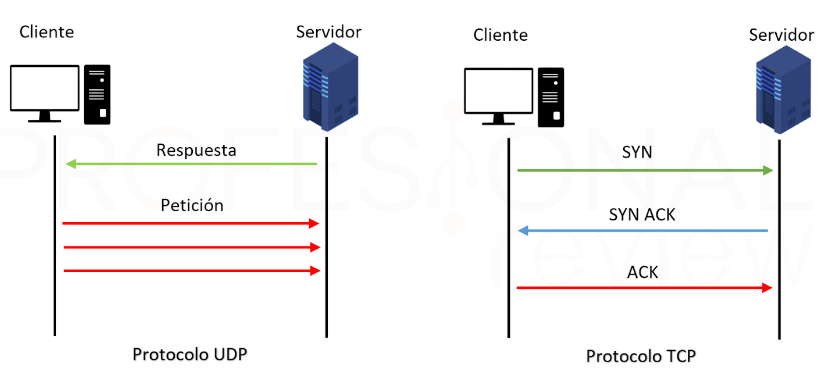
\includegraphics[width=1\textwidth]{tcp-udp.png}
	\caption{Comparativa TCP - UDP}
	\label{fig:super}
\end{figure}


En el siguiente cuadro se muestran los protocolos del nivel 7 más comunes de Internet
junto con el número de puerto que emplean.

\cite{osi}En la siguiente imagen se muestran las capas del modelo OSI:

\begin{figure}[H]
	\center
	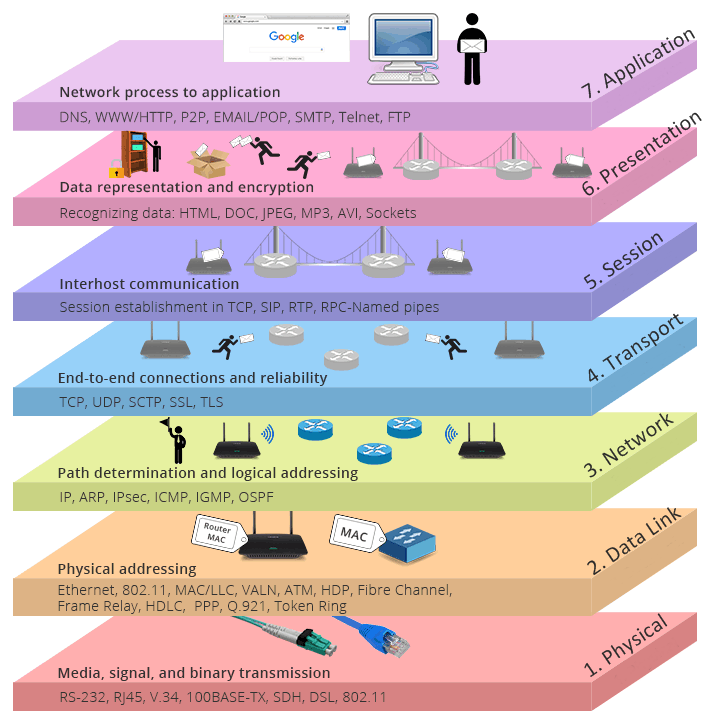
\includegraphics[width=0.7\textwidth]{osi.png}
	\caption{Modelo OSI}
	\label{fig:super}
\end{figure}

\begin{remark}
Véa el siguiente vídeo: Guerreros de la red \\
\url{https://youtu.be/1c2U1R8XXvA}
\end{remark}

\section{Arquitecturas cliente/servidor} \index{Arquitectura cliente/servidor}

\cite{sl}Las aplicaciones web son un tipo especial de aplicaciones cliente/servidor. Antes de
aprender a programar aplicaciones web conviene conocer las características básicas de las
arquitecturas cliente/servidor.

Cliente/servidor es una arquitectura de red
en la que cada ordenador o proceso en
la red es cliente o servidor
. Normalmente, los servidores son ordenadores potentes
dedicados a gestionar unidades de disco (servidor de ficheros), impresoras (servidor de impresoras), tráco de red (servidor de red), datos (servidor de bases de datos) o
incluso aplicaciones (servidor de aplicaciones), mientras que los clientes son máquinas
menos potentes y usan los recursos que ofrecen los servidores.

Esta arquitectura implica la existencia de una relación entre procesos que solicitan
servicios (clientes) y procesos que responden a estos servicios (servidores). Estos
dos tipos de procesos pueden ejecutarse en el mismo procesador o en distintos.

La arquitectura cliente/servidor permite la creación de aplicaciones distribuidas.
La principal ventaja de esta arquitectura es que facilita la separación de las funciones
según su servicio, permitiendo situar cada función en la plataforma más adecuada
para su ejecución. Además, también presenta las siguientes ventajas:

\begin{itemize}
	\item Las redes de ordenadores permiten que múltiples procesadores puedan ejecutar
	partes distribuidas de una misma aplicación, logrando concurrencia de procesos.
	\item Existe la posibilidad de migrar aplicaciones de un procesador a otro con modificaciones mínimas en los programas.
	\item Se obtiene una escalabilidad de la aplicación. Permite la ampliación horizontal
	o vertical de las aplicaciones. La \textbf{escalabilidad horizontal} se refiere a la capacidad de añadir o suprimir estaciones de trabajo que hagan uso de la aplicación
	(clientes), sin que afecte sustancialmente al rendimiento general, La \textbf{escalabilidad vertical} se refiere a la capacidad de migrar hacia servidores
	de mayor capacidad o velocidad, o de un tipo distinto de arquitectura sin que
	afecte a los clientes.
	\item Posibilita el acceso a los datos independientemente de donde se encuentre el
usuario.
\end{itemize}	

\begin{figure}[H]
	\center
	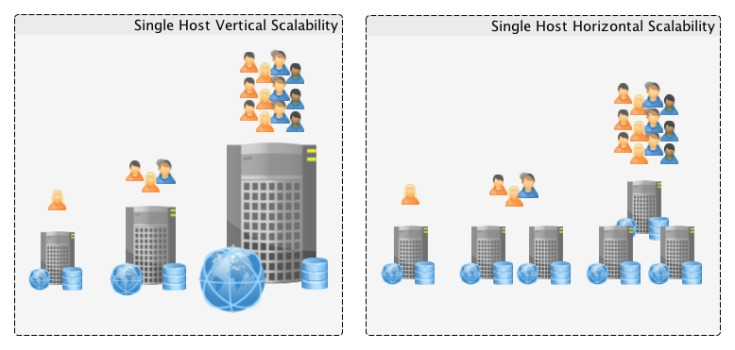
\includegraphics[width=1\textwidth]{escalar.jpeg}
	\caption{Escalamiento horizontal vs vertical}
	\label{fig:super}
\end{figure}

\subsection{Separación de funciones}\index{Separación de funciones}

La arquitectura cliente/servidor nos permite la separación de funciones en tres
niveles:

\begin{itemize}
\item \textbf{Lógica de presentación}. Se encarga de la entrada y salida de la aplicación con
el usuario. Sus principales tareas son: obtener información del usuario, enviar la
información del usuario a la lógica de negocio para su procesamiento, recibir los
resultados del procesamiento de la lógica de negocio y presentar estos resultados
al usuario.

\item \textbf{Lógica de negocio (o aplicación).} Se encarga de gestionar los datos a nivel
de procesamiento. Actúa de puente entre el usuario y los datos. Sus principales
tareas son: recibir la entrada del nivel de presentación, interactuar con la lógica
de datos para ejecutar las reglas de negocio (business rules) que tiene que cumplir la aplicación (facturación, cálculo de nóminas, control de inventario, etc.) y
enviar el resultado del procesamiento al nivel de presentación.


\item \textbf{Lógica de datos.} Se encarga de gestionar los datos a nivel de almacenamiento.
Sus principales tareas son: almacenar los datos, recuperar los datos, mantener
los datos y asegurar la integridad de los datos.
\end{itemize}	

\begin{figure}[H]
	\center
	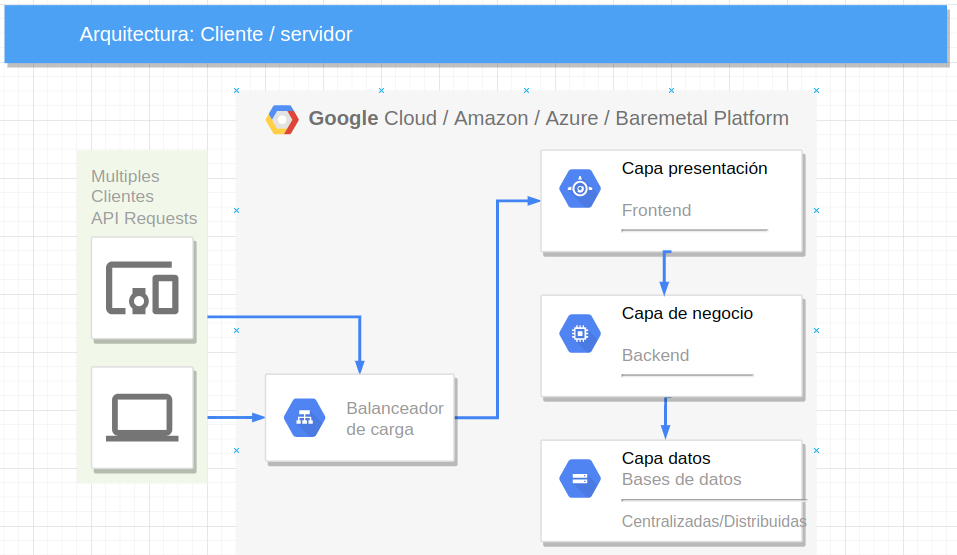
\includegraphics[width=1\textwidth]{arquitectura-cliente-servidor.png}
	\caption{Arquitectura cliente/servidor}
	\label{fig:super}
\end{figure}

\subsection{El cliente}
\cite{mdn}El cliente es cualquier herramienta que actué en representación del usuario para solicitar a
un servidor web el envío de los recursos que desea obtener mediante HTTP. Esta función es realizada en la mayor parte de los casos por un navegador Web. Hay excepciones, como el caso de programas específicamente usados por desarrolladores para desarrollar y depurar sus aplicaciones. 

El navegador es siempre el que inicia una comunicación (petición), y el servidor nunca la comienza (hay algunos mecanismos que permiten esto, pero no son muy habituales).  

Para poder mostrar una página Web, el navegador envía una petición de documento HTML al servidor. Entonces procesa este documento, y envía más peticiones para solicitar scripts, hojas de estilo (CSS), y otros datos que necesite (normalmente vídeos y/o imágenes). El navegador, une todos estos documentos y datos, y compone el resultado final: la página Web. Los scripts, los ejecuta también el navegador, y también pueden generar más peticiones de datos en el tiempo, y el navegador, gestionará y actualizará la página Web en consecuencia. 

Una página Web, es un documento de hipertexto (HTTP), luego habrá partes del texto en la página que puedan ser enlaces (links) que pueden ser activados (normalmente al hacer click sobre ellos) para hacer una petición de una nueva página Web, permitiendo así dirigir su agente de usuario y navegar por la Web. El navegador, traduce esas direcciones en peticiones de HTTP, e interpretara y procesará las respuestas HTTP, para presentar al usuario la página Web que desea.

La parte cliente de las aplicaciones web suele estar formada por el código HTML
que forma la página web más algo de código ejecutable realizado en lenguaje de script
del navegador (JavaScript o VBScript) o mediante pequeños programas (applets) realizados en Java. También se solían emplear plugins que permiten visualizar otros
contenidos multimedia (como Macromedia Flash
), aunque no se encuentran tan extendidos como las tecnologías anteriores y plantean problemas de incompatibilidad
entre distintas plataformas. Por tanto, la misión del cliente web es interpretar las
páginas HTML y los diferentes recursos que contienen (imágenes, sonidos, etc.).

\newpage

\begin{wrapfigure}{r}{0.5\textwidth}
	\begin{center}
		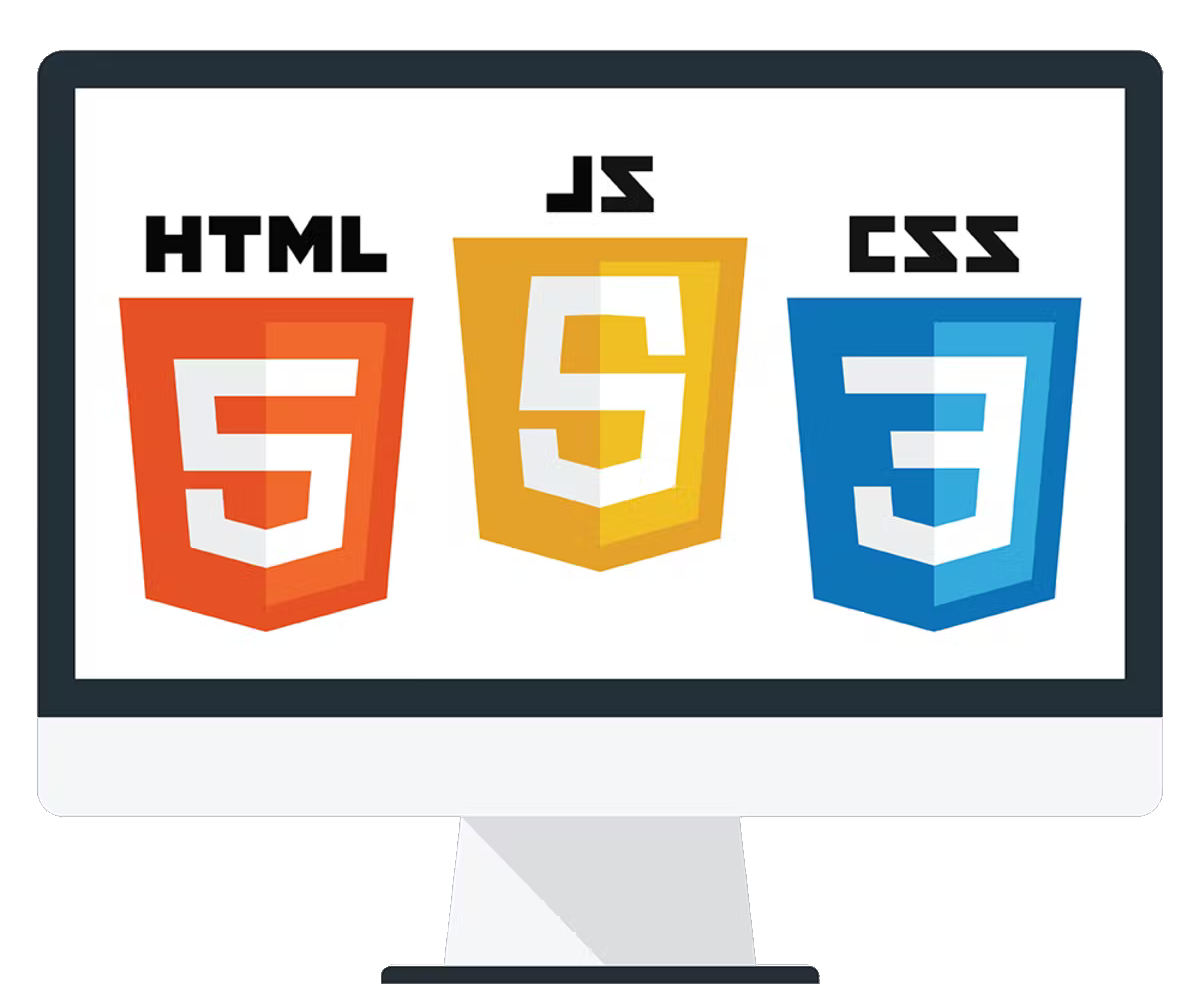
\includegraphics[width=0.3\textwidth]{cliente.png}
	\end{center}
	\caption{Cliente}
\end{wrapfigure}

Las tecnologías que se suelen emplear para programar el cliente web son:

\begin{itemize}
	\item HTML
	\item CSS
	\item Javascript
\end{itemize}

\begin{remark}
	Cada tecnología puede tener sus variantes.\\
	WebAssembly es un proyecto prometedor.\\
	Algunas tecnologías ya están en desuso (Applets, Flash entre otras.)
\end{remark}

\subsection{El servidor}

\begin{wrapfigure}{l}{0.45\textwidth}
	\begin{center}
		
\includegraphics[width=0.45\textwidth]{servidor.jpeg}
	\end{center}
	\caption{Sala de servidores}
	\label{wrap-fig:1}
\end{wrapfigure}

Al otro lado del canal de comunicación, está el servidor, el cual "sirve" los datos que ha pedido el cliente. Un servidor conceptualmente es una unica entidad, aunque puede estar formado por varios elementos, que se reparten la carga de peticiones, (load balancing), u otros programas, que gestionan otros computadores (como cache, bases de datos, servidores de correo electrónico, ...), y que generan parte o todo el documento que ha sido pedido. 

Un servidor no tiene que ser necesariamente un único equipo físico, aunque si que varios servidores pueden estar funcionando en un único computador. En el estándar HTTP/1.1 y Host , pueden incluso compartir la misma dirección de IP.

\subsection{Transferencia de páginas web a través de http}

El proceso completo, desde que el usuario solicita una página, hasta que el cliente
web (navegador) se la muestra con el formato apropiado, es el siguiente:

\begin{enumerate}
	\item El usuario especifica en el cliente web la dirección de la página que desea consultar: el usuario escribe en el navegador la dirección (URL) de la página que
	desea visitar o pulsa un enlace.
	\item El cliente establece una conexión con el servidor web.
	\item El cliente solicita la página o el objeto deseado. 
	\item El servidor envía dicha página u objeto (o, si no existe, devuelve un código de
	error).
	\item Si se trata de una página HTML, el cliente inicia sus labores de interpretación
	de los códigos HTML. Si el cliente web encuentra instrucciones que hacen referencia a otros objetos que se tienen que mostrar con la página (imágenes, sonidos, animaciones multimedia, etc.), establece automáticamente comunicación
	con el servidor web para solicitar dichos objetos.
	\item Se cierra la conexión entre el cliente y el servidor.
	\item Se muestra la página al usuario.
\end{enumerate}
	
Obsérvese que siempre se libera la conexión, por lo que ésta sólo tiene la duración
correspondiente a la transmisión de la página solicitada. Esto se hace así para no
desperdiciar innecesariamente el ancho de banda de la red mientras el usuario lee la
página recibida.
Cuando el usuario activa un enlace de la página, se establece una nueva conexión
para recibir otra página o elemento multimedia. Por ello, el usuario tiene la sensación
de que está disfrutando de una conexión permanente cuando realmente no es así.
Un detalle importante es que para cada objeto que se transfiere por la red se realiza
una conexión independiente. Por ejemplo, si el cliente web solicita una página que
contiene dos imágenes integradas, se realizan tres conexiones: una para el documento
HTML y dos para los archivos de las imágenes.

Una aplicación web (web-based application) es un tipo especial de aplicación cliente/servidor, donde tanto el cliente (el navegador, explorador o visualizador/browser)
) como
el servidor (el servidor web) y el protocolo mediante el que se comunican (HTTP)
están estandarizados y no han de ser creados por el programador de aplicaciones.

El protocolo HTTP forma parte de la familia de protocolos de comunicaciones
TCP/IP, que son los empleados en Internet. Estos protocolos permiten la conexión
de sistemas heterogéneos, lo que facilita el intercambio de información entre distintos
ordenadores. HTTP se sitúa en el nivel 7 (aplicación) del modelo OSI.


\section{HTTP/HTTPS}

\cite{mdn}Hypertext Transfer Protocol (HTTP) (o Protocolo de Transferencia de Hipertexto en español) es un protocolo de la capa de aplicación para la transmisión de documentos hipermedia, como HTML. Fue diseñado para la comunicación entre los navegadores y servidores web, aunque puede ser utilizado para otros propósitos también. Sigue el clásico modelo cliente-servidor, en el que un cliente establece una conexión, realizando una petición a un servidor y espera una respuesta del mismo. Se trata de un protocolo sin estado, lo que significa que el servidor no guarda ningún dato (estado) entre dos peticiones. Aunque en la mayoría de casos se basa en una conexión del tipo TCP/IP, puede ser usado sobre cualquier capa de transporte segura o de confianza, es decir, sobre cualquier protocolo que no pierda mensajes silenciosamente, tal como UDP.

Clientes y servidores se comunican intercambiando mensajes individuales (en contraposición a las comunicaciones que utilizan flujos continuos de datos). Los mensajes que envía el cliente, normalmente un navegador Web, se llaman peticiones, y los mensajes enviados por el servidor se llaman respuestas.

\begin{figure}[H]
	\center
	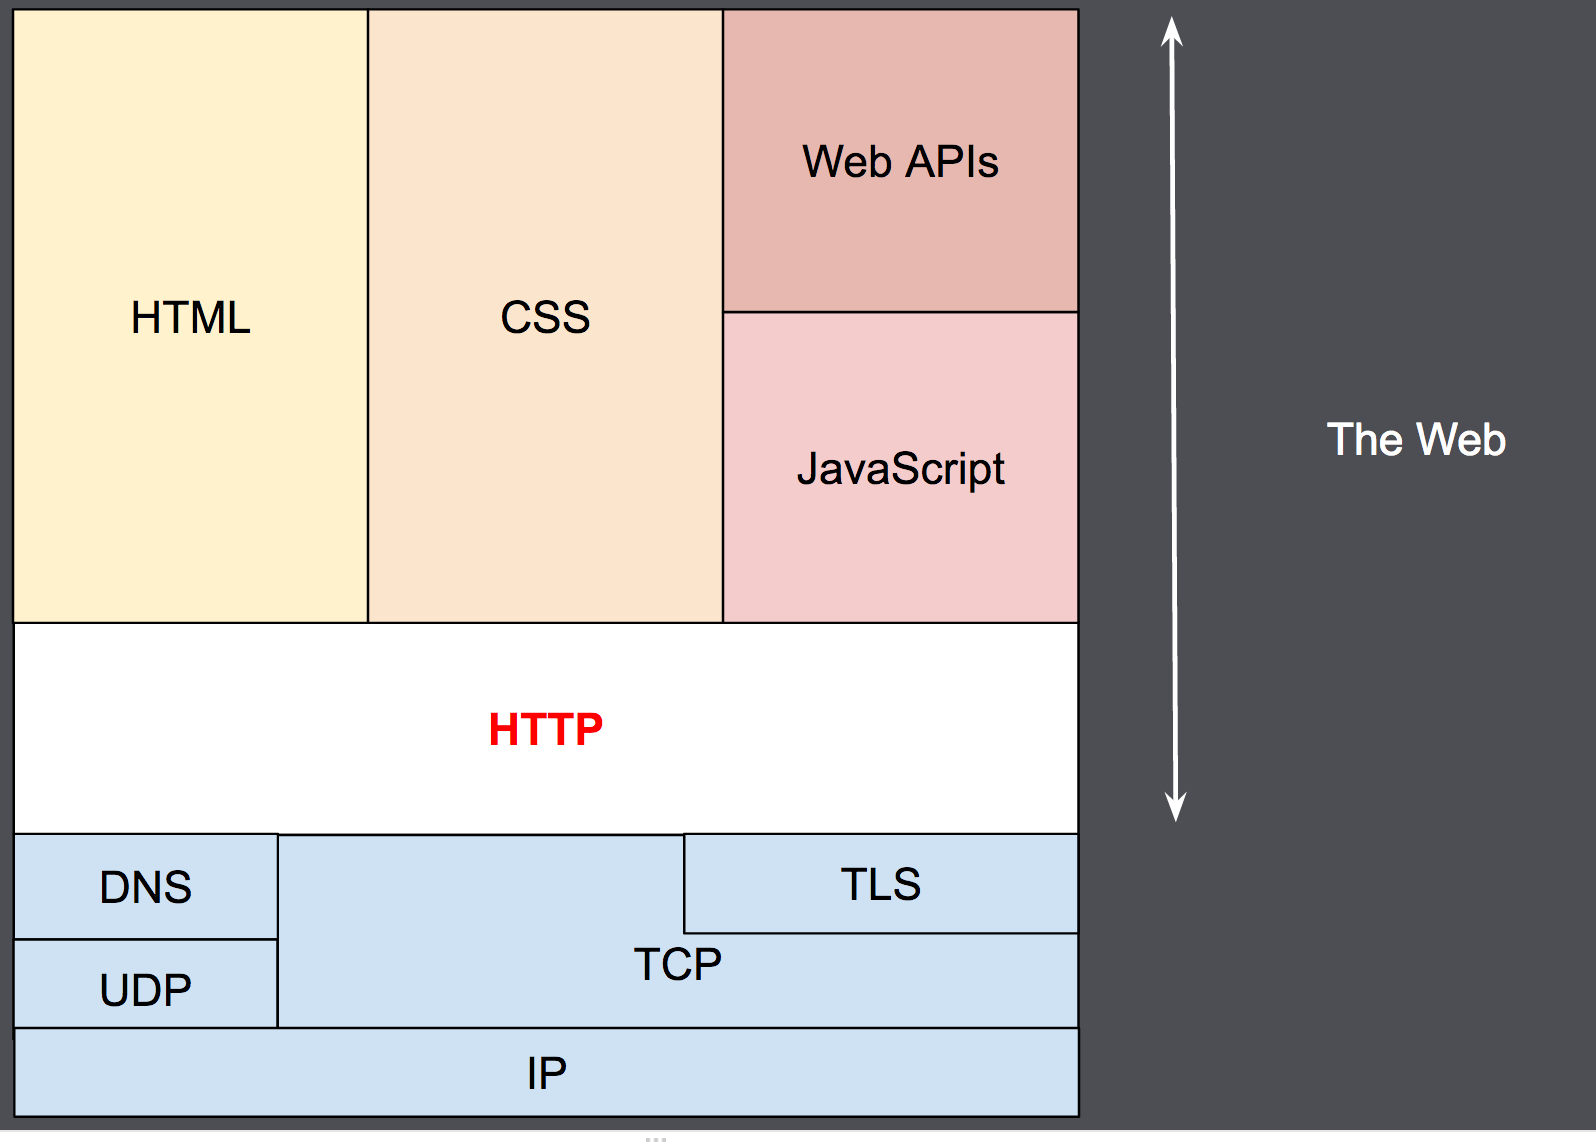
\includegraphics[width=0.5\textwidth]{HTTPyCapas.png}
	\caption{HTTP y capas}
	\label{fig:super}
\end{figure}

Diseñado a principios de la década de 1990, HTTP es un protocolo ampliable, que ha ido evolucionando con el tiempo. Es lo que se conoce como un protocolo de la capa de aplicación, y se transmite sobre el protocolo TCP, o el protocolo encriptado TLS (en-US), aunque teóricamente podría usarse cualquier otro protocolo fiable. Gracias a que es un protocolo capaz de ampliarse, se usa no solo para transmitir documentos de hipertexto (HTML), si no que además, se usa para transmitir imágenes o vídeos, o enviar datos o contenido a los servidores, como en el caso de los formularios de datos. HTTP puede incluso ser utilizado para transmitir partes de documentos, y actualizar páginas Web en el acto.

En realidad, hay más elementos intermedios, entre un navegador y el servidor que gestiona su petición: hay otros tipos de dispositivos: como routers, modems ... Es gracias a la arquitectura en capas de la Web, que estos intermediarios, son transparentes al navegador y al servidor, ya que HTTP se apoya en los protocolos de red y transporte. HTTP es un protocolo de aplicación, y por tanto se apoya sobre los anteriores. Aunque para diagnosticar problemas en redes de comunicación, las capas inferiores son irrelevantes para la definición del protocolo HTTP . 

\subsection{Características clave del protocolo HTTP}
\begin{itemize}
	\item \textbf{HTTP es sencillo}: HTTP esta pensado y desarrollado para ser leído y fácilmente interpretado por las personas, haciendo de esta manera más facil la depuración de errores, y reduciendo la curva de aprendizaje para las personan que empieza a trabajar con él.
	\item \textbf{HTTP es extensible}: Presentadas en la versión HTTP/1.0, las cabeceras de HTTP, han hecho que este protocolo sea fácil de ampliar y de experimentar con él. Funcionalidades nuevas pueden desarrollarse, sin más que un cliente y su servidor, comprendan la misma semántica sobre las cabeceras de HTTP.
	\item \textbf{HTTP es un protocolo con sesiones, pero sin estados}: HTTP es un protocolo sin estado, es decir: no guarda ningún dato entre dos peticiones en la mísma sesión. Esto crea problemáticas, en caso de que los usuarios requieran interactuar con determinadas páginas Web de forma ordenada y coherente, por ejemplo, para el uso de "cestas de la compra" en páginas que utilizan en comercio electrónico. Pero, mientras HTTP ciertamente es un protocolo sin estado, el uso de HTTP cookies, si permite guardar datos con respecto a la sesión de comunicación. Usando la capacidad de ampliación del protocolo HTTP, las cookies permiten crear un contexto común para cada sesión de comunicación.
	\item \textbf{HTTP y conexiones:} Una conexión se gestiona al nivel de la capa de trasporte, y por tanto queda fuera del alcance del protocolo HTTP. Aún con este factor, HTTP no necesita que el protocolo que lo sustenta mantenga una conexión continua entre los participantes en la comunicación, solamente necesita que sea un protocolo fiable o que no pierda mensajes (como mínimo, en todo caso, un protocolo que sea capaz de detectar que se ha pedido un mensaje y reporte un error). De los dos protocolos más comunes en Internet, TCP es fiable, mientras que UDP, no lo es. Por lo tanto HTTP, se apoya en el uso del protocolo TCP, que está orientado a conexión, aunque una conexión continua no es necesaria siempre. \\
	Todavía hoy se sigue investigando y desarrollando para conseguir un protocolo de transporte más conveniente para el HTTP. Por ejemplo, Google está experimentado con QUIC, que se apoya en el protocolo UDP y presenta mejoras en la fiabilidad y eficiencia de la comunicación. 
\end{itemize}
\subsection{¿Qué se puede controlar con HTTP?}
Se presenta a continuación una lista con los elementos que se pueden controlar con el protocolo HTTP:
\begin{itemize}
	\item \textbf{Cache}: El como se almacenan los documentos en la caché, puede ser especificado por HTTP. El servidor puede indicar a los proxies y clientes, que quiere almacenar y durante cuanto tiempo. Aunque el cliente, también puede indicar a los proxies de caché intermedios que ignoren el documento almacenado.
	\item \textbf{Flexibilidad del requisito de origen} Para prevenir invasiones de la privacidad de los usuarios, los navegadores Web, solamente permiten a páginas del mismo origen, compartir la información o datos. Esto es una complicación para el servidor, asi que mediante cabeceras HTTP, se puede flexibilizar o relajar esta división entre cliente y servidor
	\item \textbf{Autentificación} Hay páginas Web, que pueden estar protegidas, de manera que solo los usuarios autorizados puedan acceder. HTTP provee de servicios básicos de autentificación, por ejemplo mediante el uso de cabeceras como:  WWW-Authenticate, o estableciendo una sesión especifica mediante el uso de  HTTP cookies. 
	\item \textbf{Proxies y  tunneling} Servidores y/o clientes pueden estar en intranets y esconder así su verdadera dirección IP a otros. Las peticiones HTTP utilizan los proxies para acceder a ellos. Pero no todos los proxies son HTTP proxies. El protocolo SOCKS, por ejemplo, opera a un nivel más bajo. Otros protocolos, como el FTP, pueden ser servidos mediante estos proxies.
	\item \textbf{Sesiones} El uso de HTTP cookies permite relacionar peticiones con el estado del servidor. Esto define las sesiones, a pesar de que por definición el protocolo HTTP es un protocolo sin estado. Esto es muy útil no sólo para aplicaciones de comercio electrónico, sino también para cualquier sitio que permita configuración al usuario.
\end{itemize}

\subsection{Mensajes HTTP}
Existen dos tipos de mensajes HTTP: peticiones y respuestas, cada uno sigue su propio formato.

Las peticiones y respuestas HTTP, comparten una estructura similar, compuesta de:

\begin{itemize}
\item Una línea de inicio ('start-line' en inglés) describiendo la petición a ser implementada, o su estado, sea de éxito o fracaso. Esta línea de comienzo, es siempre una única línea.
\item Un grupo opcional de cabeceras HTTP, indicando la petición o describiendo el cuerpo ('body' en inglés) que se incluye en el mensaje. 
\item Una línea vacía ('empty-line' en inglés) indicando toda la meta-información ha sido enviada.
\item Un campo de cuerpo de mensaje opcional ('body' en inglés) que lleva los datos asociados con la petición (como contenido de un formulario HTML), o los archivos o documentos asociados a una respuesta (como una página HTML, o un archivo de audio, vídeo ... ) . La presencia del cuerpo y su tamaño es indicada en la línea de inicio y las cabeceras HTTP.
\end{itemize}

La línea de inicio y las cabeceras HTTP, del mensaje, son conocidas como la cabeza de la peticiones, mientras que su contenido en datos se conoce como el cuerpo del mensaje.

\begin{figure}[H]
	\center
	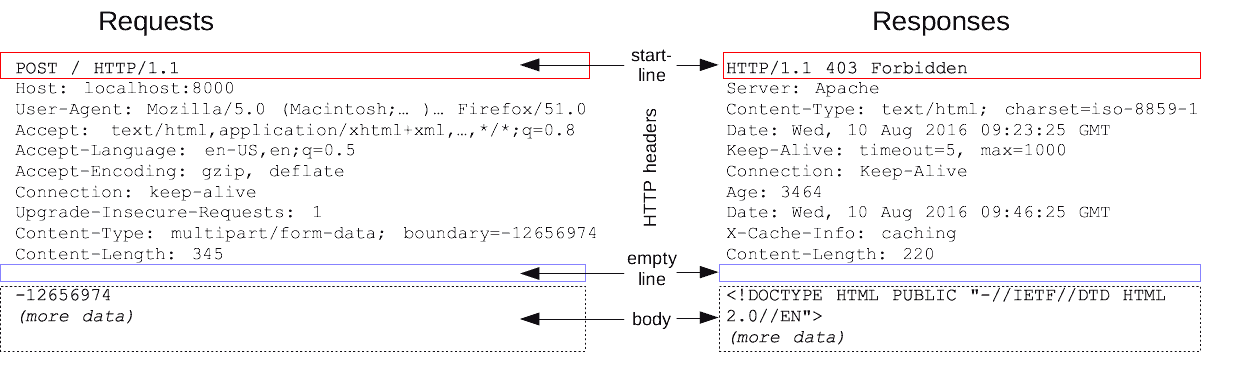
\includegraphics[width=1\textwidth]{HTTPMsgStructure2.png}
	\caption{Mensajes}
	\label{fig:super}
\end{figure}

\subsubsection{Cabeceras}

Las cabeceras HTTP  de una petición siguen la misma estructura que la de una cabecera HTTP. Una cadena de caracteres, que no diferencia mayusculas ni minusculas, seguida por dos puntos  (':')  y un valor cuya estructura depende de la cabecera. La cabecera completa, incluido el valor, ha de ser formada en una única línea, y pude ser bastante larga. 

Hay bastantes cabeceras posibles. Estas se pueden clasificar en varios grupos: 
\begin{itemize}
	\item Cabeceras generales, ('General headers' en inglés), como Via (en-US),  afectan al mensaje como una unidad completa.
	\item Cabeceras de petición, ('Request headers' en inglés), como User-Agent, Accept-Type, modifican la petición especificándola en mayor detalle ( como: Accept-Language (en-US), o dándole un contexto, como:  Referer, o restringiéndola condicionalmente, como: If-None.
	\item Cabeceras de entidad, ('Entity headers' en ingles), como Content-Length las cuales se aplican al cuerpo de la petición. Por supuesto, esta cabecera no necesita ser transmitida si el mensaje no tiene cuerpo ('body' en inglés). 
\end{itemize}

\begin{figure}[H]
	\center
	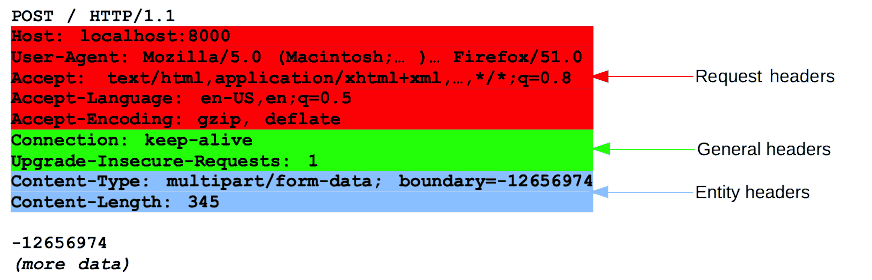
\includegraphics[width=0.7\textwidth]{HTTP_Request_Headers2.png}
	\caption{Cabeceras}
	\label{fig:super}
\end{figure}

\subsubsection{Cuerpo}
La parte final de la petición el el cuerpo. No todas las peticiones llevan uno: las peticiones que reclaman datos, como GET, HEAD, DELETE, o OPTIONS, normalmente, no necesitan ningún cuerpo. Algunas peticiones pueden mandar peticiones al servidor con el fin de actualizarlo: como es el caso con la petición POST  (que contiene datos de un formulario HTML). 
\\
Los cuerpos pueden ser dividos en dos categorias:
\begin{itemize}
	\item Cuerpos con un único dato, que consisten en un único archivo defindo por las dos cabeceras: Content-Type y Content-Length.  
	\item Cuerpos con múltiples datos, que están formados por distintos contenidos, normalmente estan asociados con los formularios HTML. 
\end{itemize}

\subsubsection{Peticiones}
Un ejemplo de petición HTTP:

\begin{figure}[H]
	\center
	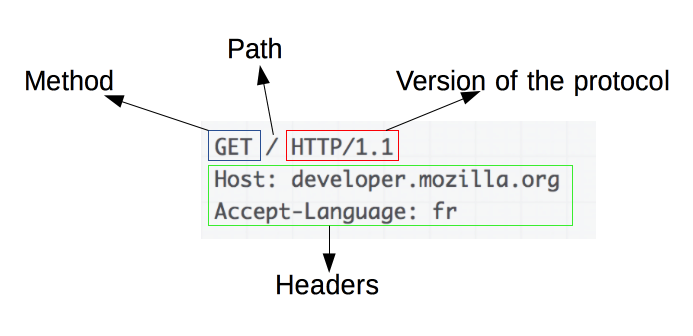
\includegraphics[width=0.5\textwidth]{HTTP_Request.png}
	\caption{Petición}
	\label{fig:super}
\end{figure}
Una petición de HTTP, está formado  por los siguientes campos:

\begin{itemize}
	\item Un método HTTP,  normalmente pueden ser un verbo, como: GET, POST o un nombre como: OPTIONS (en-US) o HEAD (en-US), que defina la operación que el cliente quiera realizar. El objetivo de un cliente, suele ser una petición de recursos, usando GET, o presentar un valor de un formulario HTML, usando POST, aunque en otras ocasiones puede hacer otros tipos de peticiones. 
	\item La dirección del recurso pedido; la URL del recurso, sin los elementos obvios por el contexto, como pueden ser: sin el  protocolo (http://),  el dominio (aquí developer.mozilla.org), o el puerto TCP (aquí el 80). 
	\item La versión del protocolo HTTP.
	\item Cabeceras HTTP opcionales, que pueden aportar información adicional a los servidores.
	\item O un cuerpo de mensaje, en algún método, como puede ser POST, en el cual envía la información para el servidor.
\end{itemize}

\subsubsection{Respuestas}
Un ejemplo de repuesta:
\begin{figure}[H]
	\center
	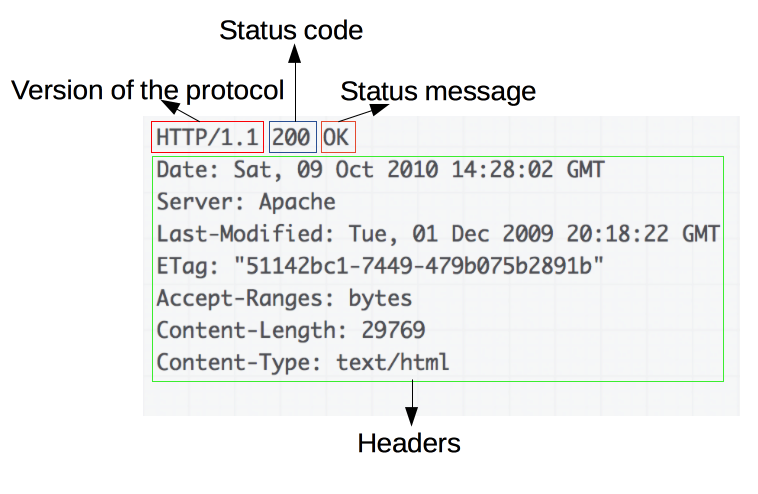
\includegraphics[width=0.5\textwidth]{HTTP_Response.png}
	\caption{Respuesta}
	\label{fig:super}
\end{figure}
Las respuestas están formadas por los siguentes campos:

\begin{itemize}
	\item La versión del protocolo HTTP que están usando.
	\item Un código de estado, indicando si la petición ha sido exitosa, o no, y debido a que. Códigos de estado muy comunes son:  200, 404, o 302
	\item Un mensaje de estado, una breve descripción del código de estado. 
	\item Cabeceras HTTP, como las de las peticiones.
	\item Opcionalmente, el recurso que se ha pedido.
\end{itemize}

\subsection{Métodos de petición HTTP}

HTTP define un conjunto de métodos de petición para indicar la acción que se desea realizar para un recurso determinado. Aunque estos también pueden ser sustantivos, estos métodos de solicitud a veces son llamados HTTP verbs. Cada uno de ellos implementan una semántica diferente, pero algunas características similares son compartidas por un grupo de ellos: ej. un request method puede ser safe, idempotent (en-US), o cacheable.

\subsubsection{GET}

El método GET  solicita una representación de un recurso específico. Las peticiones que usan el método GET sólo deben recuperar datos.

\begin{figure}[H]
	\center
	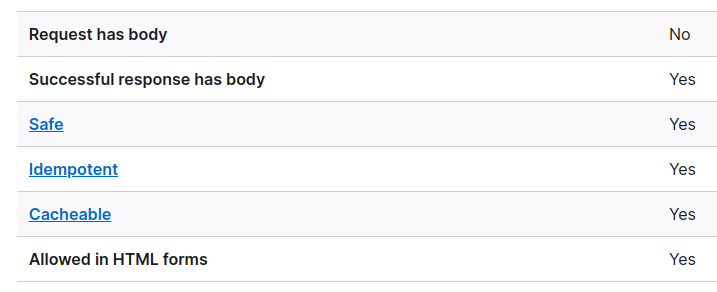
\includegraphics[width=0.7\textwidth]{get.png}
	\caption{GET}
	\label{fig:super}
\end{figure}

\subsubsection{HEAD}
El método HEAD pide una respuesta idéntica a la de una petición GET, pero sin el cuerpo de la respuesta.

\subsubsection{POST}
El método POST se utiliza para enviar una entidad a un recurso en específico, causando a menudo un cambio en el estado o efectos secundarios en el servidor. \\
El tipo de cuerpo de la solicitud se indica mediante el encabezado Content-Type.

\begin{figure}[H]
	\center
	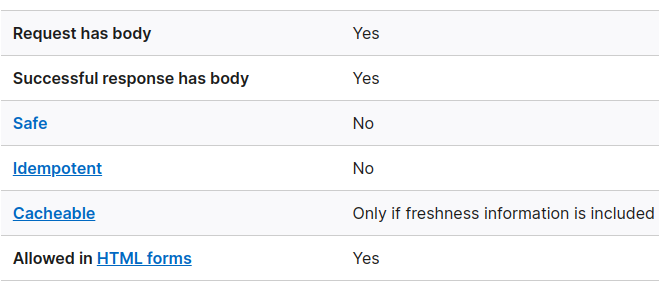
\includegraphics[width=0.7\textwidth]{post.png}
	\caption{POST}
	\label{fig:super}
\end{figure}

\subsubsection{PUT}
El método de solicitud HTTP PUT crea un nuevo recurso o reemplaza una representación del recurso de destino con la carga útil de la solicitud.

La diferencia entre PUT y POST es que PUT es idempotente: llamarlo una o varias veces sucesivamente tiene el mismo efecto (eso no es un efecto secundario), mientras que las sucesivas solicitudes POST idénticas pueden tener efectos adicionales, como realizar un pedido varias veces.
\begin{figure}[H]
	\center
	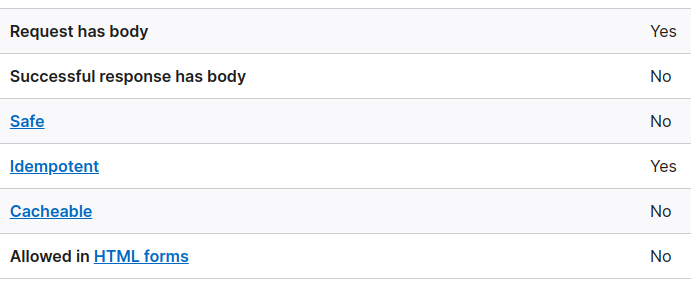
\includegraphics[width=0.7\textwidth]{put.png}
	\caption{PUT}
	\label{fig:super}
\end{figure}

\subsubsection{DELETE}
El método DELETE borra un recurso en específico.
\begin{figure}[H]
	\center
	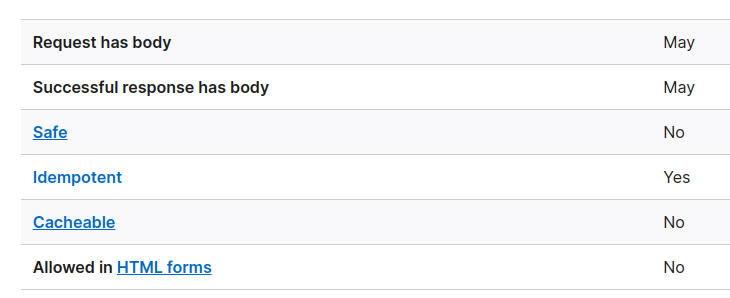
\includegraphics[width=0.7\textwidth]{delete.png}
	\caption{DELETE}
	\label{fig:super}
\end{figure}

\subsubsection{PATCH}
El método PATCH  es utilizado para aplicar modificaciones parciales a un recurso.\\
PATCH es algo análogo al concepto de "actualización" que se encuentra en CRUD (en general, HTTP es diferente a CRUD y no se deben confundir los dos).
\begin{figure}[H]
	\center
	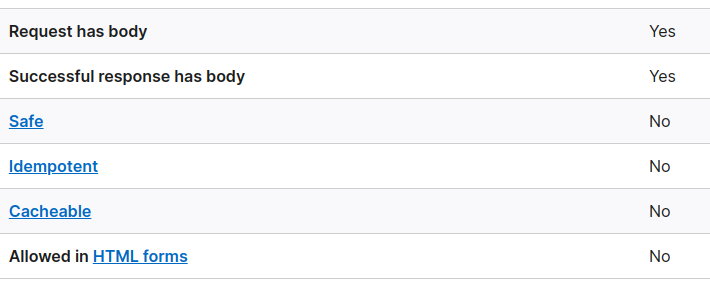
\includegraphics[width=0.7\textwidth]{patch.png}
	\caption{PATHC}
	\label{fig:super}
\end{figure}


\begin{remark}
Un método HTTP es seguro si no altera el estado del servidor. En otras palabras, un método es seguro si conduce a una operación de solo lectura. Varios métodos HTTP comunes son seguros: GET, HEAD u OPTIONS. Todos los métodos seguros también son idempotentes, pero no todos los métodos idempotentes son seguros. Por ejemplo, PUT y DELETE son idempotentes pero inseguros.
\end{remark}

\begin{remark}
Una respuesta almacenable en caché es una respuesta HTTP que se puede almacenar en caché, que se almacena para recuperarla y usarla más tarde, guardando una nueva solicitud en el servidor. No todas las respuestas HTTP se pueden almacenar en caché
\end{remark}

\begin{remark}
Un método HTTP es idempotente si se puede realizar una solicitud idéntica una o varias veces seguidas con el mismo efecto y dejando el servidor en el mismo estado. En otras palabras, un método idempotente no debería tener efectos secundarios (excepto para llevar estadísticas). Implementados correctamente, los métodos GET, HEAD, PUT y DELETE son idempotentes, pero no el método POST. Todos los métodos seguros también son idempotentes.
\end{remark}

\subsection{HTTP response status codes}

Los códigos de estado de respuesta HTTP indican si una solicitud HTTP específica se completó con éxito. Las respuestas se agrupan en cinco clases:

\begin{enumerate}
	\item Respuestas informativas (100–199)
	\item Respuestas exitosas (200–299)
	\item Mensajes de redirección (300–399)
	\item Respuestas de error del cliente (400–499)
	\item Respuestas de error del servidor (500–599)
\end{enumerate}

\subsubsection{Respuestas informativas}

\begin{itemize}
	\item 100 Continue: indica que todo está bien hasta el momento y que el cliente debe continuar con la solicitud o ignorarla si ya finalizó.
	\item 101 Protocolos de conmutación: este código se envía en respuesta a un encabezado de solicitud de actualización del cliente e indica el protocolo al que se está cambiando el servidor.
	\item 102 Procesamiento (WebDAV): Este código indica que el servidor ha recibido y está procesando la solicitud, pero aún no hay respuesta disponible.
\end{itemize}

\subsubsection{Respuestas satisfactorias}

\begin{itemize}
	\item 200 Ok: La solicitud ha tenido éxito. El significado de un éxito varía dependiendo del método HTTP.
	\item 201 Created: La solicitud ha tenido éxito y se ha creado un nuevo recurso como resultado de ello. Ésta es típicamente la respuesta enviada después de una petición PUT.
	\item 202 Accepted: La solicitud se ha recibido, pero aún no se ha actuado. Es una petición "sin compromiso", lo que significa que no hay manera en HTTP que permite enviar una respuesta asíncrona que indique el resultado del procesamiento de la solicitud. Está pensado para los casos en que otro proceso o servidor maneja la solicitud, o para el procesamiento por lotes.
\end{itemize}

\subsubsection{Redirecciones}

\begin{itemize}
	\item 300 Multiple Choice: Esta solicitud tiene más de una posible respuesta. User-Agent o el usuario debe escoger uno de ellos. No hay forma estandarizada de seleccionar una de las respuestas.
	\item 301 Moved Permanently: Este código de respuesta significa que la URI  del recurso solicitado ha sido cambiado. Probablemente una nueva URI sea devuelta en la respuesta.
\end{itemize}

\subsubsection{Errores de cliente}

\begin{itemize}
	\item 400 Bad Request: Esta respuesta significa que el servidor no pudo interpretar la solicitud dada una sintaxis inválida.
	\item 401 Unauthorized: Es necesario autenticar para obtener la respuesta solicitada. Esta es similar a 403, pero en este caso, la autenticación es posible.
	\item 403 Forbidden: El cliente no posee los permisos necesarios para cierto contenido, por lo que el servidor está rechazando otorgar una respuesta apropiada.
	\item 404 Not Found: El servidor no pudo encontrar el contenido solicitado. Este código de respuesta es uno de los más famosos dada su alta ocurrencia en la web.
\end{itemize}

\subsubsection{Errores de servidor}

\begin{itemize}
	\item 500 Internal Server Error: El servidor ha encontrado una situación que no sabe cómo manejarla.
	\item 501 Not Implemented: El método solicitado no está soportado por el servidor y no puede ser manejado
	\item 502 Bad Gateway: Esta respuesta de error significa que el servidor, mientras trabaja como una puerta de enlace para obtener una respuesta necesaria para manejar la petición, obtuvo una respuesta inválida.
	\item 503 Service Unavailable: El servidor no está listo para manejar la petición. Causas comunes puede ser que el servidor está caído por mantenimiento o está sobrecargado. Hay que tomar en cuenta que junto con esta respuesta, una página usuario-amigable explicando el problema debe ser enviada.
\end{itemize}

\subsection{URL - URI}

La «Uniform Resource Locator» (URL o Localizadora Uniforme de Recursos en Español) es una cadena de texto que especifica dónde se puede encontrar un recurso (como una página web, una imagen o un video) en Internet.

En el contexto de HTTP, las URLs se denominan "dirección web" o "enlace". Tu navegador muestra las URLs en su barra de direcciones, por ejemplo: https://developer.mozilla.org — Algunos navegadores muestran solo la parte de una URL después de "//", es decir, el Nombre de dominio.

Las URLs también se pueden utilizar para la transferencia de archivos (FTP), correos electrónicos (SMTP) y otras aplicaciones.

Un URI (Identificador Uniforme de Recursos de sus siglas en inglés: Uniform Resource Identifier) es una cadena que se refiere a un recurso. Los más comunes son URLs, que identifican el recurso dando su ubicación en la Web. URNs (en-US), por el contrario, se refiere a un recurso por un nombre, en un espacio de nombres determinados, como el ISBN(International Standard Book Number) de un libro.

Una URL está compuesta de diferentes partes, algunas obligatorias y otras opcionales. Veamos las partes más importantes usando la siguiente URL:

\begin{lstlisting}
	http://www.example.com:80/path/to/myfile.html?key1=value1&key2=value2#Somewhere
\end{lstlisting}

\begin{figure}[H]
	\center
	
\includegraphics[width=0.5\textwidth]{mdn-url-protocol1.png}
	\caption{Protocolo}
\end{figure}

http es el protocolo. La primera parte de la URL indica qué protocolo debe usar el navegador. Un protocolo es un método establecido para intercambiar o transferir datos alrededor de una red informática. Por lo general, para sitios web es el protocolo HTTP o su versión segura, HTTPS. La Web requiere uno de estos dos, pero los navegadores también saben cómo manejar otros protocolos como mailto: (para abrir un cliente de correo) o ftp: para manejar la transferencia de archivos, así que no se sorprenda si ve tales protocolos.

\begin{figure}[H]
	\center
	
\includegraphics[width=0.5\textwidth]{mdn-url-domain.png}
	\caption{Dominio}
\end{figure}

www.example.com es el nombre de dominio o autoridad que gobierna el espacio de nombres. Indica cuando es solicitado el servidor Web

\begin{figure}[H]
	\center
	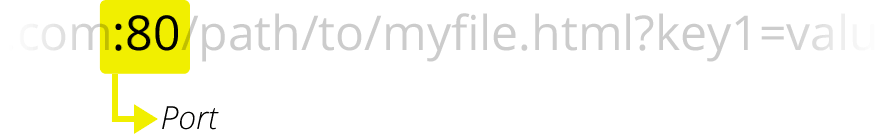
\includegraphics[width=0.5\textwidth]{mdn-url-port.png}
	\caption{Puerto}
\end{figure}

:80 es el puerto en este caso. Indica la técnica \textbf{puerta} usada para acceder a los recursos en el servidor web. Usualmente es omitido si el servidor web usa los puertos estándares del protocolo HTTP (80 para HTTP y 443 para HTTPS) para permitir el acceso a sus recursos. De lo contrario, es obligatorio.

\begin{figure}[H]
	\center
	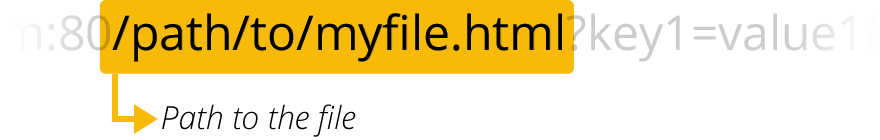
\includegraphics[width=0.5\textwidth]{mdn-url-path.png}
	\caption{Puerto}
\end{figure}

/path/to/myfile.html es la ruta de acceso al recurso en el servidor Web. En los primeros días de la Web, una ruta como esta presentaba la ubicación física del archivo en el servidor Web. Hoy en día, es sobre todo una abstracción manejada por los servidores Web sin ningún tipo de realidad física.

\begin{figure}[H]
	\center
	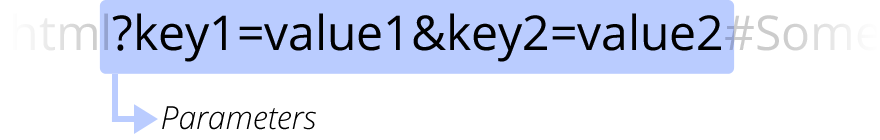
\includegraphics[width=0.5\textwidth]{mdn-url-parameters.png}
	\caption{Parametros}
\end{figure}

?key1=value1\&key2=value2 son unos parámetros adicionales proporcionados al servidor Web. Esos parámetros son una lista de pares llave/valores separados por el símbolo \&. El servidor Web puede utilizar estos parámetros para hacer cosas adicionales antes de retornar el recurso al usuario. 

\begin{figure}[H]
	\center
	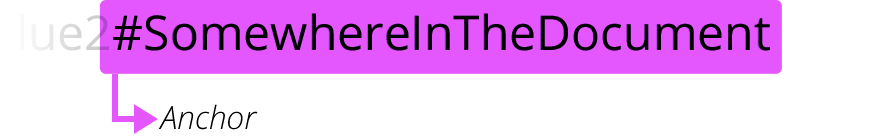
\includegraphics[width=0.5\textwidth]{mdn-url-anchor.png}
	\caption{Ancla}
\end{figure}

\#SomewhereInTheDocument es una referencia a otra parte del propio recurso. Esto representa una especie de "marcador" dentro del recurso, otorgandole al navegador las instrucciones para mostrar el contenido que se encuentra en esa referencia señalada. 

\section{Modelo de Objetos de Documento - DOM}

El DOM (Document Object Model en español Modelo de Objetos del Documento) es una API definida para representar e interactuar con cualquier documento HTML o XML. El DOM es un modelo de documento que se carga en el navegador web y que representa el documento como un árbol de nodos, en donde cada nodo representa una parte del documento (puede tratarse de un elemento, una cadena de texto o un comentario).

\begin{remark}
Una Interfaz de Programación de Aplicaciones (API, por sus siglas en inglés) define un conjunto de directivas que pueden ser usadas para tener una pieza de software funcionando con algunas otras.
\end{remark}

El DOM es una de las APIs más usadas en la Web, pues permite ejecutar código en el navegador para acceder e interactuar con cualquier nodo del documento. Estos nodos pueden crearse, moverse o modificarse. Pueden añadirse a estos nodos manejadores de eventos (event listeners en inglés) que se ejecutarán/activarán cuando ocurra el evento indicado en este manejador.

El DOM surgió a partir de la implementación de JavaScript en los navegadores. A esta primera versión también se la conoce como DOM 0 o "Legacy DOM". Hoy en día el grupo WHATWG es el encargado de actualizar el estándar de DOM.


\section{REST}

\cite{mdn}El término "Transferencia de Estado Representacional" (REST) representa un conjunto de características de diseño de arquitecturas software que aportan confiabilidad, eficiencia y escalibilidad a los sistemas distribuidos. Un sistema es llamado RESTful cuando se ajusta a estas características.

La idea básica de REST es que un recurso, e.j. un documento, es transferido con su estado y su relaciones (hipertexto) mediante formatos y operaciones estandarizadas bien definidas.

Como HTTP, el protocolo estandar de la Web, también transfiere documentos e hipertexto, las APIs HTTP a veces son llamadas APIs RESTful, servicios RESTful, o simplemente servicios REST, aunque no se ajusten del todo a la deficinición de REST. Los principiantes pueden pensar que una API REST es un servicio HTTP que puede ser llamado mediante librerias y herramientas web estandar.

\cite{redhat}REST no es un protocolo ni un estándar, sino más bien un conjunto de límites de arquitectura. Los desarrolladores de las API pueden implementarlo de distintas maneras.

Cuando el cliente envía una solicitud a través de una API de RESTful, esta transfiere una representación del estado del recurso requerido a quien lo haya solicitado o al extremo. La información se entrega por medio de HTTP en uno de estos formatos: JSON (JavaScript Object Notation), HTML, XLT, Python, PHP o texto sin formato. JSON es el lenguaje de programación más popular, ya que tanto las máquinas como las personas lo pueden comprender y no depende de ningún lenguaje, a pesar de que su nombre indique lo contrario. 

También es necesario tener en cuenta otros aspectos. Los encabezados y los parámetros también son importantes en los métodos HTTP de una solicitud HTTP de la API de RESTful, ya que contienen información de identificación importante con respecto a los metadatos, la autorización, el identificador uniforme de recursos (URI), el almacenamiento en caché, las cookies y otros elementos de la solicitud. Hay encabezados de solicitud y de respuesta, pero cada uno tiene sus propios códigos de estado e información de conexión HTTP.

Para que una API se considere de RESTful, debe cumplir los siguientes criterios:

\begin{itemize}
	\item Arquitectura cliente-servidor compuesta de clientes, servidores y recursos, con la gestión de solicitudes a través de HTTP.
	\item Comunicación entre el cliente y el servidor sin estado, lo cual implica que no se almacena la información del cliente entre las solicitudes de GET y que cada una de ellas es independiente y está desconectada del resto.
	\item Datos que pueden almacenarse en caché y optimizan las interacciones entre el cliente y el servidor.
	\item Una interfaz uniforme entre los elementos, para que la información se transfiera de forma estandarizada.
	\item Un sistema en capas que organiza en jerarquías invisibles para el cliente cada uno de los servidores (los encargados de la seguridad, del equilibrio de carga, etc.) que participan en la recuperación de la información solicitada.
	\item Código disponible según se solicite (opcional), es decir, la capacidad para enviar códigos ejecutables del servidor al cliente cuando se requiera, lo cual amplía las funciones del cliente. 
\end{itemize}

\begin{figure}[H]
	\center
	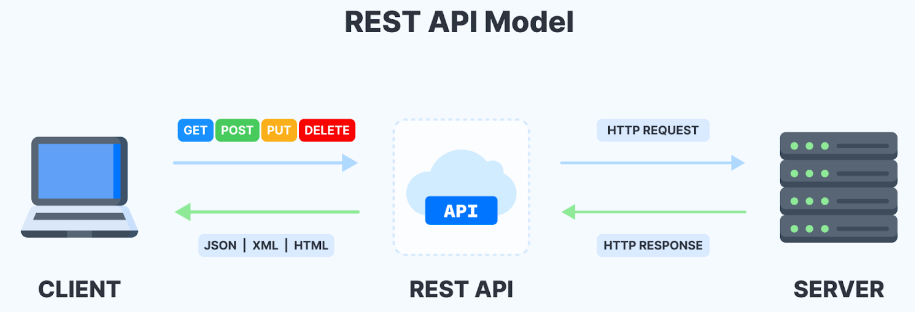
\includegraphics[width=1\textwidth]{restapimodel.png}
	\caption{REST API Model}
	\label{fig:super}
\end{figure}

REST es un conjunto de pautas que pueden implementarse según sea necesario. Por esta razón, las API de REST son más rápidas y ligeras, cuentan con mayor capacidad de ajuste y, por ende, resultan ideales para el Internet de las cosas (IoT) y el desarrollo de aplicaciones para dispositivos móviles. 


\section{Gestor de contenidos}

\cite{mdn}Un sistema de gestión de contenidos o CMS es un programa informático que permite a los usuarios publicar, organizar, cambiar o eliminar diferentes tipos de contenido como texto, imágenes incrustadas, vídeo, audio y código interactivo.

\cite{wiki}Cuenta con una interfaz que controla una o varias bases de datos donde se aloja el contenido del sitio web. El sistema permite manejar de manera independiente el contenido y el diseño. Así, es posible manejar el contenido y darle en cualquier momento un diseño distinto al sitio web sin tener que darle formato al contenido de nuevo, además de permitir la fácil y controlada publicación en el sitio a varios editores. Un ejemplo clásico es el de editores que cargan el contenido al sistema y otro de nivel superior (moderador o administrador) que permite que estos contenidos sean visibles a todo el público (los aprueba).

\subsection{Características de un CMS}
Los sistemas de gestión de contenidos se definen por las siguientes particularidades, muchas de las cuales son, a su vez, grandes ventajas:

\begin{itemize}
	\item Uso intuitivo y fácil para simplificar la edición y publicación de contenidos. No se requieren conocimientos de programación.
	\item Configuración flexible y personalizada a través de múltiples opciones.
	\item Velocidad y rendimiento elevados gracias a su excelente capacidad para el desarrollo de tareas.
	\item Seguridad presente gracias a opciones como aprobación de contenido, verificación de correo electrónico, historial de login o registro de auditoría, entre otras.
	\item Medios de soporte para ayudar a los usuarios a la resolución de dudas y problemas.
\end{itemize}

\begin{figure}[H]
	\center
	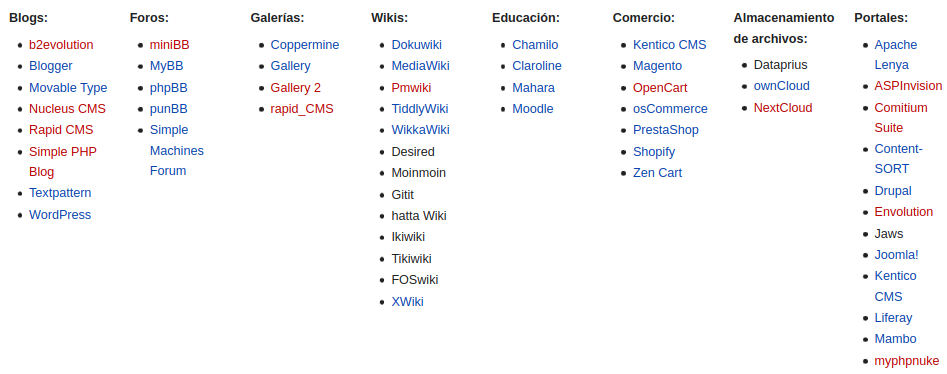
\includegraphics[width=1\textwidth]{cms1.png}
	\caption{Algunos sistemas gestores de contenido}
	\label{fig:super}
\end{figure}

\begin{figure}[H]
	\center
	
\includegraphics[width=0.7\textwidth]{cms2.png}
	\caption{Otros sistemas gestores de contenido populares}
	\label{fig:super}
\end{figure}

\section{HTML}

\cite{mdn} El Lenguaje de Marcado de Hipertexto (HTML) es el código que se utiliza para estructurar y desplegar una página web y sus contenidos. Por ejemplo, sus contenidos podrían ser párrafos, una lista con viñetas, o imágenes y tablas de datos

HTML no es un lenguaje de programación; es un lenguaje de marcado que define la estructura de tu contenido. HTML consiste en una serie de elementos que usarás para encerrar diferentes partes del contenido para que se vean o comporten de una determinada manera. Las etiquetas de encierre pueden hacer de una palabra o una imagen un hipervínculo a otro sitio, se pueden cambiar palabras a cursiva, agrandar o achicar la letra, etc. Por ejemplo, toma la siguiente línea de contenido:

\begin{lstlisting}
Mi gato es muy gruñon
\end{lstlisting}

Si quieres especificar que se trata de un párrafo, podrías encerrar el texto con la etiqueta de párrafo (<p>):

\begin{lstlisting}
	<p>Mi gato es muy gruñon</p>
\end{lstlisting}

\subsection{Anatomía de un elemento HTML}
Explora este párrafo en mayor profundidad.

\begin{figure}[H]
	\center
	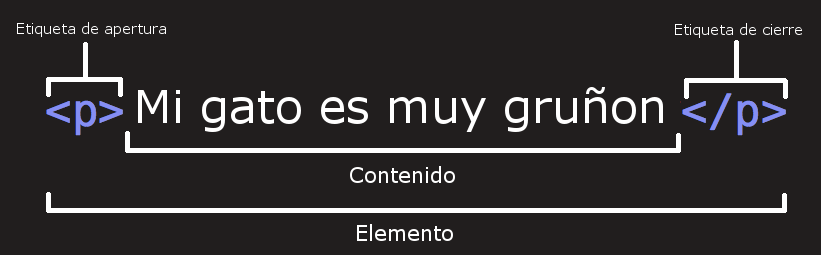
\includegraphics[width=0.7\textwidth]{htmlexp.png}
	\caption{Estructura de un elemento html}
\end{figure}

Las partes principales del elemento son:

\begin{itemize}
	\item La etiqueta de apertura: consiste en el nombre del elemento (en este caso, p), encerrado por paréntesis angulares (< >) de apertura y cierre. Establece dónde comienza o empieza a tener efecto el elemento —en este caso, dónde es el comienzo del párrafo—.
	\item El contenido: Este es el contenido del elemento. En este ejemplo, es el texto del párrafo.
	\item La etiqueta de cierre: Es lo mismo que la etiqueta de apertura, excepto que incluye una barra diagonal antes del nombre del elemento. Esto indica dónde termina el elemento; en este caso, dónde finaliza el párrafo. No incluir una etiqueta de cierre es un error común de principiante, y puede conducir a extraños resultados.
\end{itemize}

\subsection{Elementos anidados}

El elemento lo conforman la etiqueta de apertura, seguida del contenido, seguido de la etiqueta de cierre.

Se pueden poner elementos dentro de otros elementos. Esto se llama anidamiento. Si quisiéramos decir que nuestro gato es muy gruñón, podríamos encerrar la palabra muy en un elemento\textbf{ <strong>} para que aparezca destacada.

\begin{lstlisting}[language=html]
<p>Mi gato es <strong>muy</strong> gruñón.</p>
\end{lstlisting}

Hay una forma correcta e incorrecta de anidar. En el ejemplo anterior, primero abrimos el elemento p, luego abrimos el elemento strong. Para un anidamiento adecuado, primero debemos cerrar el elemento strong, antes de cerrar el p.

El siguiente es un ejemplo de la forma incorrecta de anidar:

\begin{lstlisting}[language=HTML]
<p>Mi gato es <strong>muy gruñón.</p></strong>
\end{lstlisting}

\subsection{Elementos de bloque y elementos en línea}
Hay dos categorías importantes de elementos en HTML — Estos son los elementos de bloque y los elementos en línea.

\begin{itemize}
	\item Los elementos de bloque forman un bloque visible en la página. Aparecerán en una línea nueva después de cualquier contenido anterior. Cualquier contenido que vaya después también aparecerá en una línea nueva. Los elementos a nivel de bloque suelen ser elementos estructurales de la página. Por ejemplo, un elemento a nivel de bloque puede representar encabezados, párrafos, listas, menús de navegación o pies de página. Un elemento a nivel de bloque no estaría anidado dentro de un elemento en línea, pero podría estar anidado dentro de otro elemento a nivel de bloque.
	\item Los elementos en línea están contenidos dentro de elementos de bloque y delimitan solo pequeñas partes del contenido del documento; (no párrafos enteros o agrupaciones de contenido) Un elemento en línea no hará que aparezca una nueva línea en el documento. Suele utilizarse con texto. Por ejemplo es el caso de un elemento <a> (hipervínculo) o elementos de énfasis como <em> o <strong>.
\end{itemize}

\begin{remark}
Nota: HTML5 redefinió las categorías de elementos: consulta Categorías de contenido de elementos. Si bien estas definiciones son más precisas y menos ambiguas que sus predecesoras, las nuevas definiciones son mucho más complicadas de entender que block e inline . Este artículo seguirá con estos dos términos.
\end{remark}

\subsection{Elementos vacíos}

\begin{wrapfigure}{r}{0.5\textwidth}
	\begin{center}
		
\includegraphics[width=0.2\textwidth]{firefox-icon.png}
	\end{center}
	\caption{Ejemplo elemento img}
\end{wrapfigure}

No todos los elementos siguen el patrón de etiqueta de apertura, contenido y etiqueta de cierre. Algunos elementos consisten solo en una etiqueta única, que se utiliza generalmente para insertar/incrustar algo en el documento en el lugar donde se le quiere incluir. Por ejemplo, el elemento <img> inserta una imagen en la página:

\begin{lstlisting}
<img src="https://raw.githubusercontent.com
/mdn/beginner-html-site/gh-pages/images
/firefox-icon.png">
\end{lstlisting}

\subsection{Atributos}

Los elementos también pueden tener atributos. Los atributos tienen este aspecto:

\begin{figure}[H]
	\center
	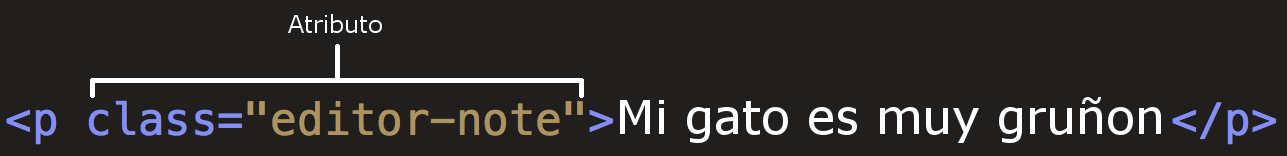
\includegraphics[width=0.7\textwidth]{htmlatributos.png}
	\caption{Atributos en un elemento html}
\end{figure}

Los atributos contienen información extra sobre el elemento que no se mostrará en el contenido. En este caso, el atributo class asigna al elemento un identificador que se puede utilizar para dotarlo de información de estilo.

Un atributo debería tener:

\begin{itemize}
	\item Un espacio entre este y el nombre del elemento. (Para un elemento con más de un atributo, los atributos también deben estar separados por espacios).
	\item El nombre del atributo, seguido por un signo igual.
	\item Un valor del atributo, rodeado de comillas de apertura y cierre.
\end{itemize}

\subsection{Anatomía de un documento HTML}

Los elementos HTML no son muy útiles por sí mismos. Ahora veremos cómo combinar los elementos individuales para formar una página HTML completa:

\begin{lstlisting}[language=html]
<!DOCTYPE html>
<html>
	<head>
		<meta charset="utf-8">
		<title>Mi página de prueba</title>
	</head>
	<body>
		<p>Esta es mi página</p>
	</body>
</html>
\end{lstlisting}

Aquí tenemos:

\begin{enumerate}}
	\item <!DOCTYPE html>: El elemento doctype. en la actualidad se ignora y se considera un legado histórico que hay que incluir para que todo funcione correctamente. <!DOCTYPE html> es la secuencia de caracteres más corta que se acepta como elemento doctype válido. 
	\item <html></html>: El elemento <html>. Este elemento envuelve todo el contenido de la página. A veces se lo conoce como el elemento raíz.
	\item <head></head>: El elemento <<head>> (cabecera). Este elemento actúa como contenedor para todos los parámetros que quieras incluir en el documento HTML que no serán visibles a los visitantes de la página. Incluye cosas como palabras clave y la descripción de la página que quieras mostrar en los resultados de búsqueda, así como la hoja de estilo para formatear nuestro contenido, declaraciones de codificación de caracteres y más. Aprenderás más acerca de esto en el siguiente artículo de la serie.
	\item <meta charset="utf-8">: Este elemento establece que tu documento HTML usará la codificación UTF-8, que incluye la gran mayoría de caracteres de todos los idiomas humanos escritos. En resumen: puede gestionar cualquier contenido textual que pongas en tu documento. No hay razón para no configurar este valor y te puede ayudar a evitar problemas más adelante.
	\item <title></title>: El elemento <title>. Este establece el título de la página, que es el título que aparece en la pestaña del navegador en la que se carga la página. El título de la página también se utiliza para describir la página cuando se marca como favorita.
	\item <body></body>: El elemento <body>. Contiene todo el contenido que quieres mostrar a los usuarios cuando visitan tu página, ya sea texto, imágenes, vídeos, juegos, pistas de audio reproducibles o cualquier otra cosa.
\end{enum+}

\section{CSS}

\cite{mdn}CSS (Cascading Style Sheets - en español Hojas de Estilo en Cascadas) es usado para darle estilo y diseño a las páginas Web — por ejemplo, para cambiar la fuente de letra, color, tamaño y el espaciado de tu contenido; dividir en múltiples columnas, o agregar animaciones y otras propiedades decorativas. Este modulo provee un inicio suave para tu ruta de aprendizaje hacia el dominio de CSS con su funcionamiento básico, como luce su sintaxis, y cómo puedes comenzar a utilizarlo y añadir estilo a HTML.

El CSS se puede usar para estilos de texto muy básicos como, por ejemplo, cambiar el color y el tamaño de los encabezados y los enlaces. Se puede utilizar para crear un diseño, como podría ser convertir una columna de texto en una composición con un área de contenido principal y una barra lateral para información relacionada. Incluso se puede usar para crear efectos de animación.

\subsection{Sintaxis del CSS}
El CSS es un lenguaje basado en reglas: cada usuario define las reglas que especifican los grupos de estilos que van a aplicarse a elementos particulares o grupos de elementos de la página web. Por ejemplo: «Quiero que el encabezado principal de mi página se muestre en letras grandes de color rojo».

El código siguiente muestra una regla CSS muy simple que proporcionaría el estilo descrito en el párrafo anterior:

\begin{lstlisting}
	h1 {
		color: red;
		font-size: 5em;
	}
\end{lstlisting}

La regla se abre con un selector (en-US). Este selecciona el elemento HTML que vamos a diseñar. En este caso, diseñaremos encabezados de nivel uno (<h1> (en-US)).

Luego tenemos un conjunto de llaves { }. Entre estas habrá una o más declaraciones, que tomarán la forma de pares de propiedad y valor. Cada par especifica cada una de las propiedades de los elementos seleccionados y el valor que queremos dar a esa propiedad.

Antes de los dos puntos, tenemos la propiedad; y después, el valor. Las propiedades (en-US) CSS admiten diferentes valores, dependiendo de qué propiedad se esté especificando. En el ejemplo anterior, tenemos la propiedad color, que puede tomar varios valores de color. También tenemos la propiedad de font-size, que puede tomar varias unidades de tamaño como valor.

Una hoja de estilo CSS contendrá muchas de estas reglas, escritas una tras otra.

\begin{lstlisting}
h1 {
	color: red;
	font-size: 5em;
}

p {
	color: black;
}
\end{lstlisting}

Algunos valores se aprenden rápidamente, mientras que otros deberán buscarse. Las páginas de propiedades individuales que hay en el proyecto MDN proporcionan una forma rápida de buscar propiedades y sus valores en caso de olvidarlos o desear saber qué más se puede usar como valor.

\begin{remark}
Nota: Puedes encontrar enlaces a todas las páginas de las propiedades CSS (junto con otras características CSS) enumeradas en la referencia CSS del proyecto MDN. Alternativamente, deberías acostumbrarte a buscar «mdn css-feature-name» en tu motor de búsqueda favorito siempre que necesites obtener más información sobre una función CSS. Por ejemplo, intenta buscar «mdn color» y «mdn font-size».
\end{remark}

\url{https://developer.mozilla.org/es/docs/Web/CSS/Reference}

\subsection{Especificaciones CSS}

Todas las tecnologías de estándares web (HTML, CSS, JavaScript, etc.) se definen en extensos documentos denominados especificaciones, publicados por organizaciones de estándares (como W3C (en-US), WHATWG, ECMA (en-US) o Khronos (en-US)) que definen con precisión cómo se supone que deben comportarse esas tecnologías.

El caso de CSS no es diferente: lo desarrolla un grupo del W3C llamado CSS Working Group. Este grupo está compuesto por representantes de proveedores de navegadores y otras compañías interesadas en CSS. También hay otras personas, conocidas como expertos invitados, que actúan como voces independientes y no están vinculados a ninguna organización.

\subsection{Agregar CSS a un documento}

Lo primero que se debe hacer es decirle al documento HTML que hay algunas reglas CSS que queremos que use. Hay tres formas diferentes de aplicar CSS a un documento HTML, sin embargo, por ahora, veremos la forma más habitual y útil de hacerlo: vincular el CSS desde el encabezado del documento.

Crea un archivo en la misma carpeta que tu documento HTML y guárdalo como styles.css. La extensión .css muestra que es un archivo CSS.

Para vincular styles.css a index.html, añade la siguiente línea en algún lugar dentro del <head> del documento HTML:

\begin{lstlisting}
<link rel="stylesheet" href="styles.css">
\end{lstlisting}

Este elemento <link> le dice al navegador que hay una hoja de estilo con el atributo rel y la ubicación de esa hoja de estilo como el valor del atributo href
\begin{remark}
	El atributo rel indica la relación del documento enlazado con el actual.
\end{remark}

Puedes determinar múltiples selectores a la vez, separándolos con una coma. Si queremos que todos los párrafos y todos los elementos de la lista sean verdes, el código se verá así:

\begin{lstlisting}
	p, li {
		color: green;
	}
\end{lstlisting}

\subsection{Añadir una clase}
Hasta ahora, hemos utilizado elementos cuyo nombre se basa en el nombre de elemento que reciben en HTML. Esto funciona siempre que se desee que todos los elementos de ese tipo tengan el mismo aspecto en el documento. La mayoría de las veces no es el caso, por lo que deberás encontrar una manera de seleccionar un subconjunto de los elementos sin que cambien los demás. La forma más común de hacer esto es añadir una clase al elemento HTML y determinarla.
\\
En tu documento HTML, añade al segundo elemento de la lista un atributo de clase. Debería verse así:
\begin{lstlisting}
<ul>
<li>Punto uno</li>
<li class = "special">Punto dos</li>
<li>Punto <em>tres</em></li>
</ul>
\end{lstlisting}
En tu CSS, puedes seleccionar una clase special creando un selector que comience con un carácter de punto final. Añade lo siguiente a tu archivo CSS:
\begin{lstlisting}
	.special {
		color: orange;
		font-weight: bold;
	}
\end{lstlisting}

Puedes aplicar la clase special a cualquier elemento de la página que desees que tenga el mismo aspecto que este elemento de lista. Por ejemplo, es posible que desees que el <span> del párrafo también sea naranja y en negrita. 

A veces verás reglas con un selector que enumera el selector de elementos HTML junto con la clase:

\begin{lstlisting}
	li.special {
		color: orange;
		font-weight: bold;
	}
\end{lstlisting}

Esta sintaxis significa «determina cualquier elemento li que tenga una clase special». Si hicieras esto, ya no podrías aplicar la clase a un elemento <span> u otro elemento simplemente añadiéndole la clase; tendrías que añadir ese elemento a la lista de selectores:

\begin{lstlisting}
	li.special,
	span.special {
		color: orange;
		font-weight: bold;
	}
\end{lstlisting}

\subsection{Dar formato según la ubicación en un documento}
Hay momentos en los que querrás que algo se vea diferente en función de dónde esté en el documento. Hay múltiples selectores que pueden hacerlo, pero por ahora veremos solo un par. En nuestro documento hay dos elementos <em>: uno dentro de un párrafo y el otro dentro de un elemento de la lista. Para seleccionar solo un <em> que esté anidado dentro de un elemento <li>, podemos usar un selector llamado combinador descendente, que simplemente toma la forma de un espacio entre otros dos selectores.

\begin{remark}
Combinador Css de descendiente: (espacio en blanco) o >>
\end{remark}

\begin{lstlisting}
	li em {
		color: rebeccapurple;
	}
\end{lstlisting}

Este selector separará cualquier elemento <em> que esté dentro de (un descendiente de) <li>. Entonces, en tu documento de ejemplo, deberías encontrar que el <em> del tercer elemento de la lista es morado, pero el que hay en el párrafo no ha cambiado.


Otra cosa que puedes probar es dar formato un párrafo que venga directamente a continuación de un título que esté en el mismo nivel de jerarquía en el HTML. Para hacerlo, coloca un + (un combinador hermano adyacente) entre los selectores.

\begin{lstlisting}
h1 + p {
	font-size: 200%;
}
\end{lstlisting}

\begin{lstlisting}
<h1>I am a level one heading</h1>

<p>This is a paragraph of text. In the text is a <span>span element</span> 
and also a <a href="http://example.com">link</a>.</p>

<p>This is the second paragraph. It contains an <em>emphasized</em> element.</p>

<ul>
<li>Item <span>one</span></li>
<li>Item two</li>
<li>Item <em>three</em></li>
</ul>
\end{lstlisting}

Salida:

\begin{figure}[H]
	\center
	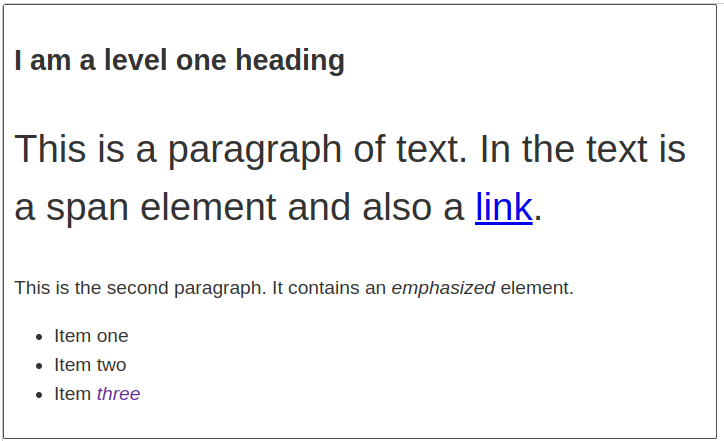
\includegraphics[width=0.7\textwidth]{css1.png}
	\caption{Salida de formato según la ubicación}
	\label{fig:super}
\end{figure}

\subsection{Dar formato según el estado}

 Un ejemplo sencillo es el estilo de los enlaces. Cuando damos formato a un enlace, necesitamos seleccionar el elemento <a> (anclaje). Tiene diferentes estados dependiendo de si se ha visitado o no, se pasa por encima, o se presiona con el teclado o se hace clic (se activa). Puedes usar CSS para dar formato a estos diferentes estados. El CSS que encontrarás a continuación presenta en color rosa los enlaces que no se han visitado y en verde los que sí.
 
 \begin{lstlisting}
a:link {
	color: pink;
}

a:visited {
	color: green;
}
 \end{lstlisting}

Puedes cambiar la apariencia del enlace, por ejemplo, eliminando el subrayado, lo que se logra mediante la siguiente regla:

 \begin{lstlisting}
	a:hover {
		text-decoration: none;
	}
\end{lstlisting}

\subsection{Estilos en línea}
Los estilos en línea son declaraciones CSS que afectan a un solo elemento, contenido dentro de un atributo de style:
\begin{lstlisting}
<!DOCTYPE html>
<html>
<head>
<meta charset="utf-8">
<title>Mi experimento CSS</title>
</head>
<body>
<h1 style="color: blue;background-color: yellow;border: 1px solid black;">¡Hola mundo!</h1>
<p style="color:red;">Este es mi primer ejemplo de CSS</p>
</body>
</html>~
\end{lstlisting}

\begin{remark}
¡No hagas esto a menos que realmente tengas que hacerlo! Es realmente malo a la hora de realizar el mantenimiento 
\end{remark}

\subsection{Selectores}
No se puede hablar de CSS sin mencionar los selectores, de los cuales ya hemos descubierto varios tipos diferentes en la lección Empezar con el CSS. Un selector es, como determinamos, un elemento de nuestro documento HTML para aplicarle estilo. Si los estilos no se aplican correctamente, es probable que el selector no coincida con lo que crees que debería coincidir.

Cada regla CSS comienza con un selector o una lista de selectores que indican al navegador a qué elemento o elementos deben aplicarse dichas reglas. Todos los siguientes son ejemplos de selectores válidos o listas de selectores.

\begin{lstlisting}
h1
a:link
.manythings
#onething
*
.box p
.box p:first-child
h1, h2, .intro
\end{lstlisting}

\begin{figure}[H]
	\center
	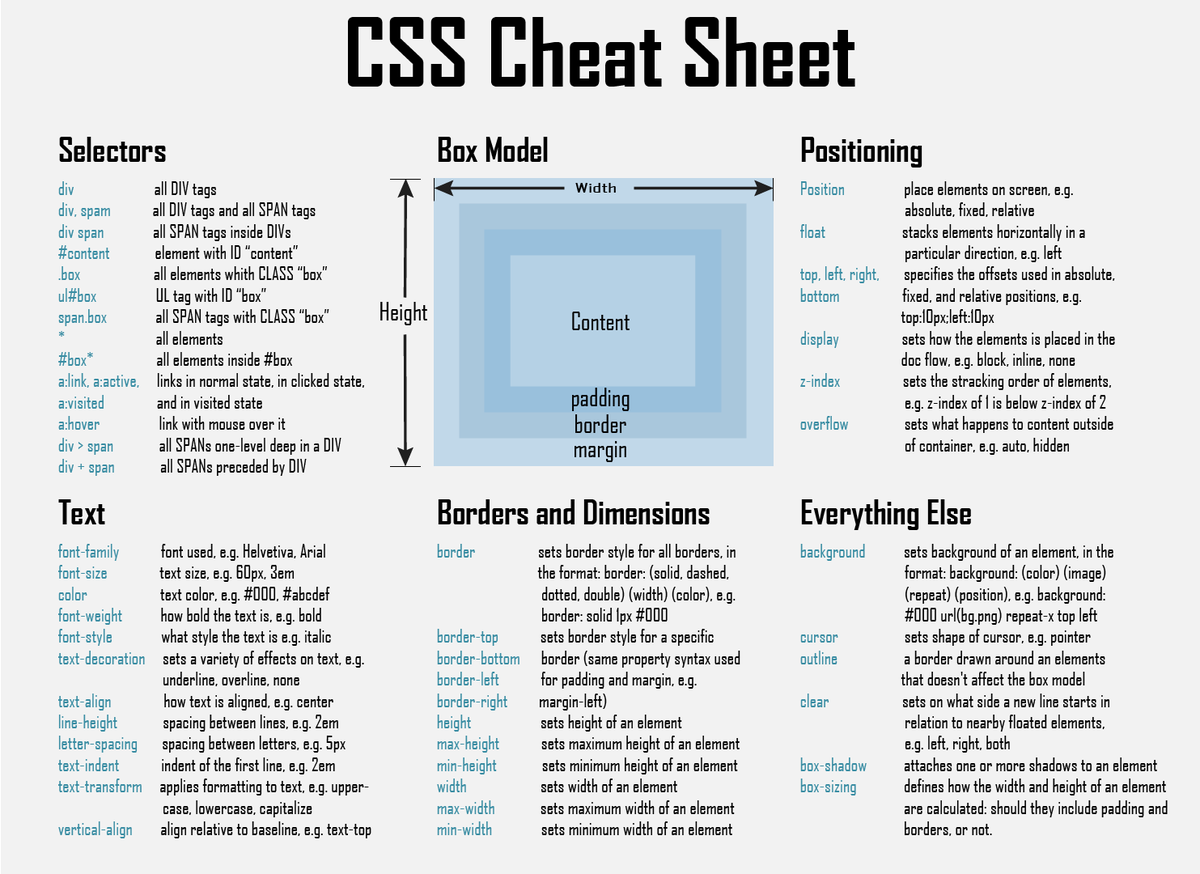
\includegraphics[width=1\textwidth]{cheatsheet-css.png}
	\caption{Hoja de trucos CSS}
	\label{fig:super}
\end{figure}

\subsection{Especificidad}
A menudo habrá situaciones en las que dos selectores podrían determinar un mismo elemento HTML. Considera la siguiente hoja de estilo, en que definimos una regla con un selector p que establecerá los párrafos en color azul, y también una clase que establecerá los elementos seleccionados en color rojo.

\begin{lstlisting}
.special {
	color: red;
}

p {
	color: blue;
}
\end{lstlisting}

Digamos que en nuestro documento HTML hay un párrafo con una clase special. Ambas reglas podrían aplicarse. ¿Cuál ganará? ¿De qué color crees que será nuestro párrafo?

\begin{lstlisting}
<p class="special">¿De qué color soy?</p>
\end{lstlisting}

El lenguaje CSS tiene reglas para controlar cuál ganará en caso de colisión; reciben el nombre de cascada y especificidad. En el siguiente bloque de códigos hemos definido dos reglas para el selector p, pero el párrafo termina siendo de color azul. Esto se debe a que la declaración que lo establece en azul aparece más abajo en la hoja de estilo, y los estilos posteriores anulan a los anteriores. Así funciona la regla de la cascada.

\subsection{@rules}
Las @rules (leído "at-rules" en inglés) dan al CSS algunas instrucciones sobre cómo comportarse. Algunas @rules son simples, con el nombre de la regla y un valor. Por ejemplo, para importar una hoja de estilo adicional a tu hoja de estilo CSS principal, puedes usar @import:

\begin{lstlisting}
@import 'styles2.css';
\end{lstlisting}

Una de las @rules más comunes con las que te encontrarás es @media, que permite usar consultas a medios para aplicar CSS solo cuando se dan ciertas condiciones (por ejemplo, cuando la resolución de la pantalla supera un valor determinado o la anchura supera un valor concreto).

En el CSS que se muestra a continuación, tenemos una hoja de estilo que le da al elemento <body> un color de fondo rosado. Sin embargo, luego usamos @media para crear una sección de nuestra hoja de estilo que solo se aplicará en los navegadores con una ventana gráfica de más de 30em de ancho. Si el navegador es más ancho que 30em, el color de fondo será azul.

\begin{lstlisting}
body {
	background-color: pink;
}

@media (min-width: 30em) {
	body {
		background-color: blue;
	}
}
\end{lstlisting}

\subsection{Abreviaturas}
Algunas propiedades como font, background, padding, border y margin se llaman propiedades abreviadas. Esto se debe a que permiten establecer varios valores de propiedad en una sola línea, lo que ahorra tiempo y ordena el código.

Por ejemplo, esta línea:

\begin{lstlisting}
/* En propiedades abreviadas con 4 valores, como margin y padding (relleno), los valores se aplican
según el orden: arriba, derecha, abajo e izquierda (en sentido horario desde la parte superior). También hay otros
tipos de abreviaturas, como las propiedades abreviadas con 2 valores que establecen el relleno/margen,
arriba/abajo, y luego izquierda/derecha */
padding: 10px 15px 15px 5px;
\end{lstlisting}

Hace lo mismo que todas estas juntas:

\begin{lstlisting}
padding-top: 10px;
padding-right: 15px;
padding-bottom: 15px;
padding-left: 5px;
\end{lstlisting}

\subsection{¿Cómo funciona realmente el CSS?}

Cuando un navegador muestra un documento, ha de combinar el contenido con la información de estilo del documento. Procesa el documento en una serie de etapas, que enumeraremos a continuación. Ten en cuenta que este es un modelo muy simplificado de lo que sucede cuando un navegador carga una página web y que cada navegador gestiona el proceso de manera diferente. Pero esto es más o menos lo que sucede.

\begin{itemize}
	\item El navegador carga el HTML (por ejemplo, lo recibe de la red).
	\item Convierte el HTML en un DOM (Modelo de objetos del documento). El DOM representa el documento en la memoria del ordenador. Lo explicaremos más detalladamente en la sección siguiente.
	\item Entonces, el navegador va a buscar la mayor parte de los recursos vinculados al documento HTML, como las imágenes y los videos incrustados... ¡y también el CSS vinculado! JavaScript aparece un poco más adelante en el proceso, pero no vamos a hablar de ello aún para evitar complicar las cosas.
	\item El navegador analiza el CSS y ordena en diferentes «cubos» las diferentes reglas según el tipo de selector. Por ejemplo, elemento, clase, ID, y así sucesivamente. Para cada tipo de selector que encuentre, calcula qué reglas deben aplicarse y a qué nodos en el DOM se les aplica el estilo según corresponda (este paso intermedio se llama árbol de renderización).
	\item El árbol de renderización presenta la estructura en que los nodos deben aparecer después de aplicarle las reglas.
	\item En la pantalla se muestra el aspecto visual de la página (esta etapa se llama pintura).
	
	
\end{itemize}
El siguiente diagrama ofrece una visión sencilla de este proceso.

\begin{figure}[H]
	\center
	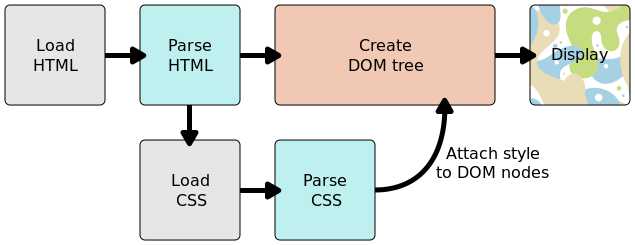
\includegraphics[width=1\textwidth]{rendering.png}
	\caption{Carga del css}
	\label{fig:super}
\end{figure}


\subsection{Normal flow}

Los elementos en las páginas web se presentan de acuerdo con el flujo normal, hasta que hacemos algo que cambie eso. Esta sección explica las bases del flujo normal para aprender como cambiarlo.

¿Cómo se presentan por defecto los elementos?

En primer lugar, se toma de las cajas de cada uno de los elementos el contenido, luego se añade cualquier área de relleno, borde y margen alrededor de ellas; es el modelo de cajas que hemos visto antes.

De manera predeterminada, el contenido de un elemento de nivel de bloque es el 100\% del ancho de su elemento padre y su altura viene determinada por su contenido. Los elementos en línea tienen su altura y anchura determinados por su contenido. No puedes establecer el ancho o la altura de los elementos en línea, simplemente se ubican dentro del contenido de los elementos de nivel de bloque. Si deseas controlar el tamaño de un elemento en línea de esta manera, debes configurarlo para que se comporte como un elemento de nivel de bloque con display: block; (o incluso, display: inline-block;, que combina características de ambos).

Esto explica los elementos individuales, pero ¿qué hay del modo como los elementos interactúan entre sí? El flujo de diseño normal (mencionado en el artículo de introducción al diseño) es el sistema mediante el cual los elementos se colocan en la ventana gráfica del navegador. De manera predeterminada, los elementos de nivel de bloque se presentan en la dirección del flujo del bloque, en función del modo de escritura de los padres (initial: horizontal-tb): cada uno aparecerá en una línea nueva debajo de la última, y estarán separados por cualquier margen que se establezca en ellos. Por lo tanto, en inglés, o en cualquier otro modo de escritura horizontal y de arriba a abajo, los elementos de nivel de bloque se disponen verticalmente.

Los elementos en línea se comportan de manera diferente: no aparecen en líneas nuevas; en su lugar, se asientan en la misma línea entre sí y con cualquier contenido de texto adyacente (o envuelto), siempre que tengan espacio dentro del ancho del elemento de nivel de bloque primario. Si no hay espacio, el texto o los elementos que desborden bajarán a la línea siguiente.

Si dos elementos adyacentes tienen algún margen configurado y los dos márgenes se tocan, se mantiene el mayor de los dos y el menor desaparece; esto se llama colapso del margen, y ya lo hemos visto antes.

\begin{figure}[H]
	\center
	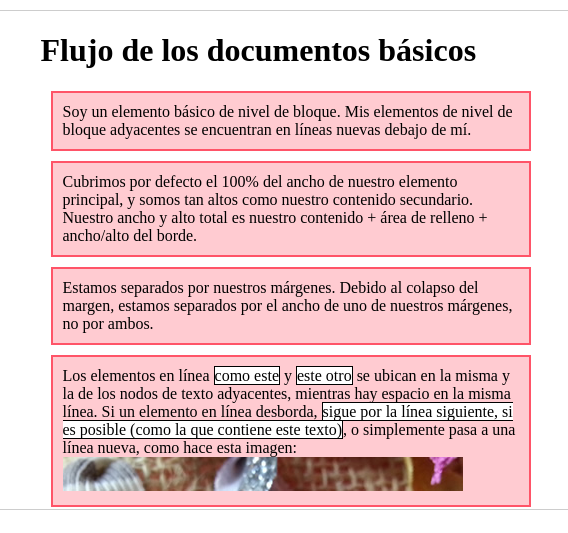
\includegraphics[width=1\textwidth]{flujo1.png}
	\caption{Ejemplo Flujo normal}
	\label{fig:super}
\end{figure}

\subsection{Contenido desbordante}


El desbordamiento es lo que sucede cuando hay demasiado contenido para caber en un contenedor. En esta guía aprenderá qué es el desbordamiento y cómo gestionarlo.

Todo en CSS es una caja. Puede restringir el tamaño de estos cuadros asignando valores de ancho y alto (o tamaño en línea y tamaño de bloque). El desbordamiento ocurre cuando hay demasiado contenido para caber en una caja. CSS proporciona varias herramientas para administrar el desbordamiento. A medida que avance con el diseño de CSS y escriba CSS, encontrará más situaciones de desbordamiento.

CSS intenta evitar la "pérdida de datos"
Consideremos dos ejemplos que demuestran el comportamiento predeterminado de CSS cuando hay desbordamiento.

El primer ejemplo es una caja que ha sido restringida estableciendo una altura. Luego agregamos contenido que excede el espacio asignado. El contenido desborda el cuadro y cae en el párrafo siguiente.


\begin{figure}[H]
	\center
	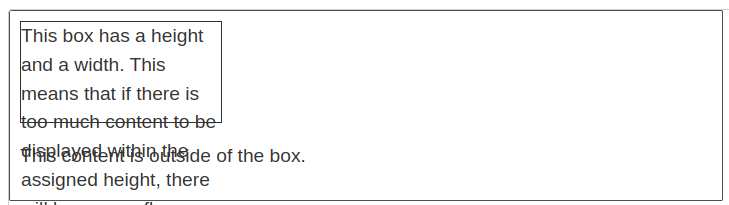
\includegraphics[width=1\textwidth]{desbordamiento1.png}
	\caption{Ejemplo desbordamiento}
	\label{fig:super}
\end{figure}

El segundo ejemplo es una palabra en un cuadro. La caja se ha hecho demasiado pequeña para la palabra, por lo que se sale de la caja.

\begin{figure}[H]
	\center
	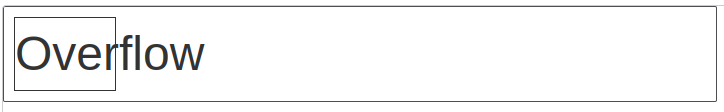
\includegraphics[width=1\textwidth]{desbordamiento2.png}
	\caption{Ejemplo desbordamiento}
	\label{fig:super}
\end{figure}

Siempre que sea posible, CSS no oculta el contenido. Esto provocaría la pérdida de datos. El problema con la pérdida de datos es que es posible que no lo notes. Es posible que los visitantes del sitio web no se den cuenta. Si el botón de enviar en un formulario desaparece y nadie puede completarlo, ¡esto podría ser un gran problema! En cambio, CSS se desborda de manera visible. Es más probable que vea que hay un problema. En el peor de los casos, un visitante del sitio le informará que el contenido se superpone.

La propiedad de desbordamiento es cómo tomas el control del desbordamiento de un elemento. Es la forma en que le indica al navegador cómo debe comportarse. El valor predeterminado de overflow es visible. Con este valor predeterminado, podemos ver el contenido cuando se desborda.

Para recortar el contenido cuando se desborda, puede establecer desbordamiento: oculto. Esto hace exactamente lo que dice: oculta el desbordamiento. Tenga en cuenta que esto puede hacer que algunos contenidos sean invisibles. Solo debe hacer esto si ocultar contenido no causará problemas.

\begin{lstlisting}
.box {
	border: 1px solid #333333;
	width: 200px;
	height: 100px;
	overflow: hidden;
}
\end{lstlisting}

\begin{figure}[H]
	\center
	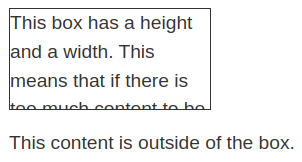
\includegraphics[width=0.6\textwidth]{desbordamiento3.png}
	\caption{Ejemplo desbordamiento}
	\label{fig:super}
\end{figure}

Usando overflow: scroll, los navegadores con barras de desplazamiento visibles siempre las mostrarán, incluso si no hay suficiente contenido para desbordar.

\begin{lstlisting}
.box {
	overflow: scroll;
}
\end{lstlisting}

\begin{remark}
Para simplemente desplazarse en el eje y, puede usar la propiedad overflow-y, configurando overflow-y: scroll. y overflow-x para desplazarse en el eje de las x
\end{remark}

\subsubsection{Flexbox}

Flexbox es un método de diseño de página unidimensional para compaginar elementos en filas o columnas. Los elementos de contenido se ensanchan para rellenar el espacio adicional y se encogen para caber en espacios más pequeños. En este artículo expondremos todas sus características básicas.

\subsubsection{Grid} \cite{mdn}

CSS Grid Layout presenta un sistema de cuadrícula bidimensional para CSS. Las cuadrículas se pueden utilizar para posicionar áreas principales de la página o pequeños elementos de la interfaz de usuario.

CSS Grid layout contiene funciones de diseño dirigidas a los desarrolladores de aplicaciones web. El CSS grid se puede utilizar para lograr muchos diseños diferentes. También se destaca por permitir dividir una página en áreas o regiones principales, por definir la relación en términos de tamaño, posición y capas entre partes de un control construido a partir de primitivas HTML.

Al igual que las tablas, el grid layout permite a un autor alinear elementos en columnas y filas. Sin embargo, con CSS grid son posibles muchos más diseños y de forma más sencilla que con las tablas. Por ejemplo, los elementos secundarios de un contenedor de cuadrícula podrían posicionarse para que se solapen y se superpongan, de forma similar a los elementos posicionados en CSS.

¿Qué es una cuadrícula(grid)?

Una cuadrícula es un conjunto de líneas horizontales y verticales que se intersectan - un grupo define columnas y el otro filas. Los elementos se pueden colocar en la cuadrícula respetando estas columnas y filas. El diseño de cuadrícula CSS tiene las siguientes características:

\begin{itemize}
	\item Tamaños fijos y flexibles:  puede crear una cuadrícula con tamaños fijos, utilizando píxeles, también se puede crear una cuadrícula utilizando tamaños flexibles con porcentajes o con la nueva unidad de medida fr (fracción), diseñada para este propósito.
	\item Posicionamiento de elementos: puede colocar elementos en una ubicación precisa en la cuadrícula utilizando números de línea, nombres o seleccionando un área de la cuadrícula.
	\item Creación de líneas adicionales para alojar contenido: Grid Layout  es lo suficientemente flexible como para permitir agregar filas y columnas adicionales cuando sea necesario.
	\item Control de alineación: contiene características de alineación para poder controlar la forma cómo se alinean los elementos una vez colocados en un área de cuadrícula y cómo está alineada toda la cuadrícula.
	\item Control de contenido superpuesto: Se puede colocar más de un elemento en una celda de la cuadrícula o área, las cuales pueden solaparse o superponerse total o parcialmente entre sí. Esta estratificación puede ser controlada con la propiedad z-index.
\end{itemize}

\begin{remark}
	Para mayor información vea: 
	\url{https://developer.mozilla.org/es/docs/Web/CSS/CSS_Grid_Layout/Basic_Concepts_of_Grid_Layout}
\end{remark}

\subsection{Frameworks CSS}

\cite{wiki} Un framework de CSS es una biblioteca de estilos genéricos que puede ser usada para implementar diseños web. Aportan una serie de utilidades que pueden ser aprovechadas frecuentemente en los distintos diseños web.

\subsubsection{Ventajas}

Un framework de CSS, si está bien diseñado e implementado, proporciona las siguientes ventajas:

\begin{itemize}
	\item Proporcionar una forma fácil y por tanto rápida de implementar diseños web.
	\item Nos aseguran que el diseño va a funcionar en una amplia gama de navegadores
	\item Nos aseguran que su código cumple cierta normas estándar.
	\item Nos aseguran cierto grado de fiabilidad en la eficacia de las utilidades que nos aportan. El framework se supone que está bien probado para asegurarnos que no hay errores.
\end{itemize}

\subsubsection{Inconvenientes}
El uso de un framework de CSS puede (no siempre) llevar aparejado las siguientes desventajas:

\begin{itemize}
	\item La importación de código del framework que no es necesario en nuestro diseño web concreto. Esto provoca un incremento innecesario del consumo del ancho de banda y del tiempo de descarga.
	\item Hay un menor control por parte del maquetador de lo que realmente está sucediendo en la visualización de la página web. Esto suele ser un problema cuando se tiene que corregir algún efecto indeseado.
	\item Al diseñar con código prehecho, podemos estar limitándonos en cuanto las posibilidades de elección del diseño web.
\end{itemize}

\subsubsection{Algunos frameworks css}

\textbf{Tailwindcss}
\url{https://tailwindcss.com/}

\textbf{Daisyui}
\url{https://daisyui.com/}

\textbf{Material UI}
\url{https://mui.com/material-ui/getting-started/overview/}

\textbf{Bulma}
\url{https://bulma.io/}

\textbf{NextUI}
\url{https://nextui.org/}

\textbf{Ant Design}
\url{https://ant.design/}

\textbf{PrimeNG}
\url{https://www.primefaces.org/primeng/}

\textbf{PrimeReact}
\url{https://www.primefaces.org/primereact/}

\textbf{Chakra}
\url{https://chakra-ui.com/}

\section{Javascript}

\subsection{ECMAScript}

\cite{ecma} Ecma International es una asociación industrial dedicada a la estandarización de los sistemas de información y comunicación.

Ecma está impulsada por miembros de la industria para satisfacer sus necesidades, brindando un panorama competitivo saludable basado en la diferenciación de productos y servicios en lugar de modelos tecnológicos, generando confianza entre los proveedores y usuarios de nuevas tecnologías.

\cite{wiki} ECMAScript es una especificación de lenguaje de programación publicada por ECMA International. El desarrollo empezó en 1996 y estuvo basado en el popular lenguaje JavaScript propuesto como estándar por Netscape Communications Corporation. Actualmente está aceptado como el estándar ISO/IEC 22275:2018.

ECMAScript define un lenguaje de tipos dinámicos ligeramente inspirado en Java y otros lenguajes del estilo de C. Soporta algunas características de la programación orientada a objetos mediante objetos basados en prototipos y pseudoclases.

\cite{ecma} Estandarización del lenguaje de programación ECMAScript® de propósito general, multiplataforma e independiente del proveedor. Esto incluye la sintaxis, la semántica y las bibliotecas del lenguaje y las tecnologías complementarias que respaldan el lenguaje. Este trabajo pretende no utilizar patentes o, de ser así, solo patentes libres de regalías.

\begin{figure}[H]
	\center
	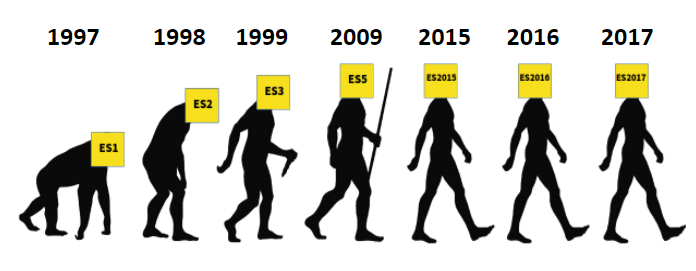
\includegraphics[width=0.6\textwidth]{ecma-evolution.png}
	\caption{Evolución Ecmascript :-)}
\end{figure}

\begin{remark}
	La versión actual del estandar EcmaScript en el momento de escribir esta guía es la 2022 y la puedes encontrar en el siguiente enlace:
	\url{https://www.ecma-international.org/wp-content/uploads/ECMA-262_13th_edition_june_2022.pdf}
\end{remark}


\subsection{Javascript}
\cite{mdn} JavaScript es un lenguaje de programación o de secuencias de comandos que te permite implementar funciones complejas en páginas web, cada vez que una página web hace algo más que sentarse allí y mostrar información estática para que la veas, muestra oportunas actualizaciones de contenido, mapas interactivos, animación de Gráficos 2D/3D, desplazamiento de máquinas reproductoras de vídeo, etc., puedes apostar que probablemente JavaScript está involucrado. Es la tercera capa del pastel de las tecnologías web estándar, dos de las cuales (HTML y CSS) hemos cubierto con mucho más detalle en otras partes del Área de aprendizaje.

El núcleo del lenguaje JavaScript de lado del cliente consta de algunas características de programación comunes que te permiten hacer cosas como:

\begin{itemize}
	\item Almacenar valores útiles dentro de variables. En el ejemplo anterior, por ejemplo, pedimos que ingreses un nuevo nombre y luego almacenamos ese nombre en una variable llamada name.
	\item Operaciones sobre fragmentos de texto (conocidas como "cadenas" (strings) en programación).
	\item Ejecuta código en respuesta a ciertos eventos que ocurren en una página web.
	\item ¡Y mucho más!
\end{itemize}

Sin embargo, lo que aún es más emocionante es la funcionalidad construida sobre el lenguaje JavaScript de lado del cliente. Las denominadas interfaces de programación de aplicaciones (API) te proporcionan superpoderes adicionales para utilizar en tu código JavaScript.

Cuando el navegador encuentra un bloque de JavaScript, generalmente lo ejecuta en orden, de arriba a abajo. Esto significa que debes tener cuidado con el orden en el que colocas las cosas.

JavaScript es un lenguaje de programación interpretado ligero. El navegador web recibe el código JavaScript en su forma de texto original y ejecuta el script a partir de ahí. Desde un punto de vista técnico, la mayoría de los intérpretes de JavaScript modernos utilizan una técnica llamada compilación en tiempo real para mejorar el rendimiento; el código fuente de JavaScript se compila en un formato binario más rápido mientras se usa el script, de modo que se pueda ejecutar lo más rápido posible. Sin embargo, JavaScript todavía se considera un lenguaje interpretado, ya que la compilación se maneja en el entorno de ejecución, en lugar de antes.

\subsection{¿Cómo agregas JavaScript a tu página?}
JavaScript se aplica a tu página HTML de manera similar a CSS. Mientras que CSS usa elementos <link> para aplicar hojas de estilo externas y elementos <style> para aplicar hojas de estilo internas a HTML, JavaScript solo necesita un amigo en el mundo de HTML: el elemento <script>.

Hay una serie de problemas relacionados con la carga de los scripts en el momento adecuado. ¡Nada es tan simple como parece! Un problema común es que todo el HTML de una página se carga en el orden en que aparece. Si estás utilizando JavaScript para manipular elementos en la página (o exactamente, el Modelo de objetos del documento (en-US)), tu código no funcionará si el JavaScript se carga y procesa antes que el HTML que estás intentando haga algo.

Una solución pasada de moda a este problema solía ser colocar tu elemento script justo en la parte inferior del cuerpo (por ejemplo, justo antes de la etiqueta </body>), para que se cargara después de haber procesado todo el HTML. El problema con esta solución es que la carga/procesamiento del script está completamente bloqueado hasta que se haya cargado el DOM HTML. En sitios muy grandes con mucho JavaScript, esto puede causar un importante problema de rendimiento y ralentizar tu sitio.

\subsubsection{async y defer}

En realidad, hay dos modernas características que podemos usar para evitar el problema del bloqueo de script: async y defer (que vimos anteriormente). Veamos la diferencia entre estas dos.

Los scripts cargados con el atributo async (ve más abajo) descargarán el script sin bloquear el renderizado de la página y lo ejecutará tan pronto como el script se termine de descargar. No tienes garantía de que los scripts se ejecuten en un orden específico, solo que no detendrán la visualización del resto de la página. Es mejor usar async cuando los scripts de la página se ejecutan de forma independiente y no dependen de ningún otro script de la página.

Los scripts cargados con el atributo defer (ve a continuación) se ejecutarán en el orden en que aparecen en la página y los ejecutará tan pronto como se descarguen el script y el contenido:

\begin{lstlisting}[language=HTML]
<script defer src="js/vendor/jquery.js"></script>

<script defer src="js/script2.js"></script>

<script defer src="js/script3.js"></script>
\end{lstlisting}

Todos los scripts con el atributo defer se cargarán en el orden en que aparecen en la página. Entonces, en el segundo ejemplo, podemos estar seguros de que jquery.js se cargará antes que script2.js y script3.js y que script2.js se cargará antes de script3.js. No se ejecutarán hasta que se haya cargado todo el contenido de la página, lo cual es útil si tus scripts dependen de que el DOM esté en su lugar (por ejemplo, modifican uno o más elementos de la página).

Para resumir:

\begin{itemize}
	\item async y defer indican al navegador que descargue los scripts en un hilo separado, mientras que el resto de la página (el DOM, etc.) se descarga, por lo que los scripts no bloquean la carga de la página.
	\item Si tus scripts se deben ejecutar inmediatamente y no tienen ninguna dependencia, utiliza async.
	\item Si tus scripts necesitan esperar a ser procesados y dependen de otros scripts y/o del DOM en su lugar, cárgalos usando defery coloca tus elementos <script> correspondientes en el orden que desees que el navegador los ejecute.
\end{itemize}

\subsection{Un poco de sintaxis}

\subsubsection{Declaraciones if ... else }
\\\\
Echemos un vistazo a la declaración condicional más común que usarás en JavaScript.

\textbf{— El humilde if ... else statement.}

Una sintaxis básica if...else luce así. pseudocode:

\begin{lstlisting}[language=javascript]
	if (condición) {
		código a ejecutar si la condicion es verdadera
	} else {
		ejecuta este otro código si la condicion es falsa
	}
\end{lstlisting}
\\
\textbf{else if}
\\
Hay una forma de encadenar  opciones / resultados adicionales extras a if...else — usando else if. Cada opción extra requiere un bloque adicional para poner en medio de bloque if() { ... } y else { ... } 

\subsubsection{Bucles}

Los lenguajes de programación son muy útiles para completar rápidamente tareas repetitivas, desde múltimples cálculos básicos hasta cualquier otra situación en donde tengas un montón de elementos de trabajo similares que completar. Aquí vamos a ver las estructuras de bucles disponibles en JavaScript que pueden manejar tales necesidades.

Los bucles de programación están relacionados con todo lo referente a hacer una misma cosa una y otra vez — que se denomina como iteración en el idioma de programación.

\textbf{El bucle estándar for}
\\
Exploremos algunos constructores de bucles específicos. El primero, que usarás la mayoría de las veces, es el bucle for - este tiene la siguiente sintaxis:

\begin{lstlisting}
for (inicializador; condición de salida; expresión final) {
	// código a ejecutar
}
\end{lstlisting}

Observa un ejemplo real para poder entender esto más claramente.

\begin{lstlisting}
var cats = ['Bill', 'Jeff', 'Pete', 'Biggles', 'Jasmin'];
var info = 'My cats are called ';
var para = document.querySelector('p');

for (var i = 0; i < cats.length; i++) {
	info += cats[i] + ', ';
}

para.textContent = info;
\end{lstlisting}

Esto nos da el siguiente resultado:

\begin{lstlisting}
My cats are called Bill, Jeff, Pete, Biggles, Jasmin,
\end{lstlisting}

\begin{remark}
Más información sobre bucles en:
\url{https://developer.mozilla.org/es/docs/Learn/JavaScript/Building_blocks/Looping_code}
\end{remark}

Por los momentos no se continua con la sintaxis de javascript, se explicarán mas conceptos desde el punto de vista de Typescript en la siguiente sección.



\section{Typescript}

\cite{type} JavaScript (también conocido como ECMAScript) comenzó su vida como un simple lenguaje de secuencias de comandos para navegadores. En el momento en que se inventó, se esperaba que se usara para fragmentos cortos de código incrustados en una página web; escribir más de unas pocas docenas de líneas de código hubiera sido algo inusual. Debido a esto, los primeros navegadores web ejecutaban dicho código con bastante lentitud. Sin embargo, con el tiempo, JS se hizo cada vez más popular y los desarrolladores web comenzaron a usarlo para crear experiencias interactivas.

Los desarrolladores de navegadores web respondieron a este mayor uso de JS optimizando sus motores de ejecución (compilación dinámica) y ampliando lo que se podía hacer con él (agregando API), lo que a su vez hizo que los desarrolladores web lo usaran aún más. En los sitios web modernos, su navegador ejecuta con frecuencia aplicaciones que abarcan cientos de miles de líneas de código. Este es un crecimiento largo y gradual de "la web", comenzando como una simple red de páginas estáticas y evolucionando hacia una plataforma para aplicaciones ricas de todo tipo.

Más que esto, JS se ha vuelto lo suficientemente popular como para usarse fuera del contexto de los navegadores, como implementar servidores JS usando node.js. La naturaleza de "ejecutar en cualquier lugar" de JS lo convierte en una opción atractiva para el desarrollo multiplataforma. ¡ Hay muchos desarrolladores en estos días que usan solo JavaScript para programar toda su pila!

Para resumir, tenemos un lenguaje que fue diseñado para usos rápidos y luego creció hasta convertirse en una herramienta completa para escribir aplicaciones con millones de líneas. Cada idioma tiene sus propias peculiaridades : rarezas y sorpresas, y el humilde comienzo de JavaScript hace que tenga muchas de ellas. Algunos ejemplos:

\begin{itemize}
	\item El operador de igualdad de JavaScript ( ==) coacciona sus argumentos, lo que genera un comportamiento inesperado:
	\begin{lstlisting}
		if ("" == 0) {
			// It is! But why??
		}
	\end{lstlisting}
	\item JavaScript también permite acceder a propiedades que no están presentes (Preste atención a \textbf{height}):
	\begin{lstlisting}[language=javascript]
		const obj = { width: 10, height: 15 };
		// Why is this NaN? Spelling is hard!
		const area = obj.width * obj.heigth;
	\end{lstlisting}
\end{itemize}

La mayoría de los lenguajes de programación arrojarían un error cuando ocurren este tipo de errores, algunos lo harían durante la compilación, antes de que se ejecute cualquier código. Al escribir programas pequeños, tales peculiaridades son molestas pero manejables; al escribir aplicaciones con cientos o miles de líneas de código, estas sorpresas constantes son un problema grave.

\subsection{TypeScript: un verificador de tipo estático}

Dijimos anteriormente que algunos lenguajes no permitirían que esos programas con errores se ejecutaran en absoluto. La detección de errores en el código sin ejecutarlo se conoce como verificación estática . Determinar qué es un error y qué no en función de los tipos de valores en los que se opera se conoce como verificación de tipos estáticos.

TypeScript verifica un programa en busca de errores antes de la ejecución, y lo hace en función de los tipos de valores , es un verificador de tipo estático . Por ejemplo, el último ejemplo anterior tiene un error debido al tipo de obj. Aquí está el error encontrado por TypeScript:

\begin{lstlisting}[language=typescript]
	const obj = { width: 10, height: 15 };
	const area = obj.width * obj.heigth;
	
	Property 'heigth' does not exist on type '{ width: number; height: number; }'. Did you mean 'height'?
\end{lstlisting}



\subsection{Un superconjunto tipado de JavaScript}

Sin embargo, ¿cómo se relaciona TypeScript con JavaScript?

Sintaxis
TypeScript es un lenguaje que es un superconjunto de JavaScript: por lo tanto, la sintaxis JS es TS legal. La sintaxis se refiere a la forma en que escribimos texto para formar un programa.

TypeScript no considera ningún código JavaScript como un error debido a su sintaxis. Esto significa que puede tomar cualquier código JavaScript que funcione y ponerlo en un archivo TypeScript sin preocuparse por cómo está escrito exactamente.

\subsection{Tipos}

TypeScript es un superconjunto tipado , lo que significa que agrega reglas sobre cómo se pueden usar diferentes tipos de valores. El error anterior acerca de obj.heigthno fue un error de sintaxis : es un error de usar algún tipo de valor (un tipo ) de manera incorrecta.

En términos generales, una vez que el compilador de TypeScript termina de verificar su código, borra los tipos para producir el código "compilado" resultante. Esto significa que una vez que se compila su código, el código JS simple resultante no tiene información de tipo.

Esto también significa que TypeScript nunca cambia el comportamiento de su programa en función de los tipos que infiere. La conclusión es que, si bien es posible que vea errores de tipo durante la compilación, el sistema de tipo en sí no influye en cómo funciona su programa cuando se ejecuta.

Finalmente, TypeScript no proporciona ninguna biblioteca de tiempo de ejecución adicional. Sus programas utilizarán la misma biblioteca estándar (o bibliotecas externas) que los programas de JavaScript, por lo que no hay un marco adicional específico de TypeScript para aprender.

\subsubsection{Primitivos}

JavaScript tiene tres primitivas muy utilizadas: string, number, y boolean. Cada una tiene un tipo correspondiente en TypeScript. Como es de esperar, estos son los mismos nombres que verías si usaras el operador typeof de JavaScript en un valor de esos tipos:

\begin{itemize}
	\item string representa valores de cadena como "Hola, mundo".
	\item number es para números como 42. JavaScript no tiene un valor especial en tiempo de ejecución para los enteros, así que no hay equivalente a int o float - todo es simplemente número.
	\item boolean es para los dos valores true y false.
\end{itemize}


\subsubsection{Arreglos}

Para especificar el tipo de un array como [1, 2, 3], puedes utilizar la sintaxis número[]; esta sintaxis funciona para cualquier tipo (por ejemplo, cadena[] es un array de cadenas, y así sucesivamente). También puedes ver esto escrito como Array<número>, que significa lo mismo.

\subsubsection{any}

TypeScript también tiene un tipo especial, any, que puedes usar siempre que no quieras que un valor particular cause errores de comprobación de tipos.

Cuando un valor es de tipo any, puedes acceder a sus propiedades (que a su vez serán de tipo any), llamarlo como una función, asignarlo a (o desde) un valor de cualquier tipo, o cualquier otra cosa que sea sintácticamente legal.

Para mayor información sobre typescript leer los siguientes apartados de documentación oficial:
\url{https://www.typescriptlang.org/docs/handbook/2/everyday-types.html}
\url{https://www.typescriptlang.org/docs/handbook/2/functions.html}
\url{https://www.typescriptlang.org/docs/handbook/2/objects.html}
\url{https://www.typescriptlang.org/docs/handbook/2/classes.html}

A continuación algunas hojas de trucos

\begin{figure}[H]
	\center
	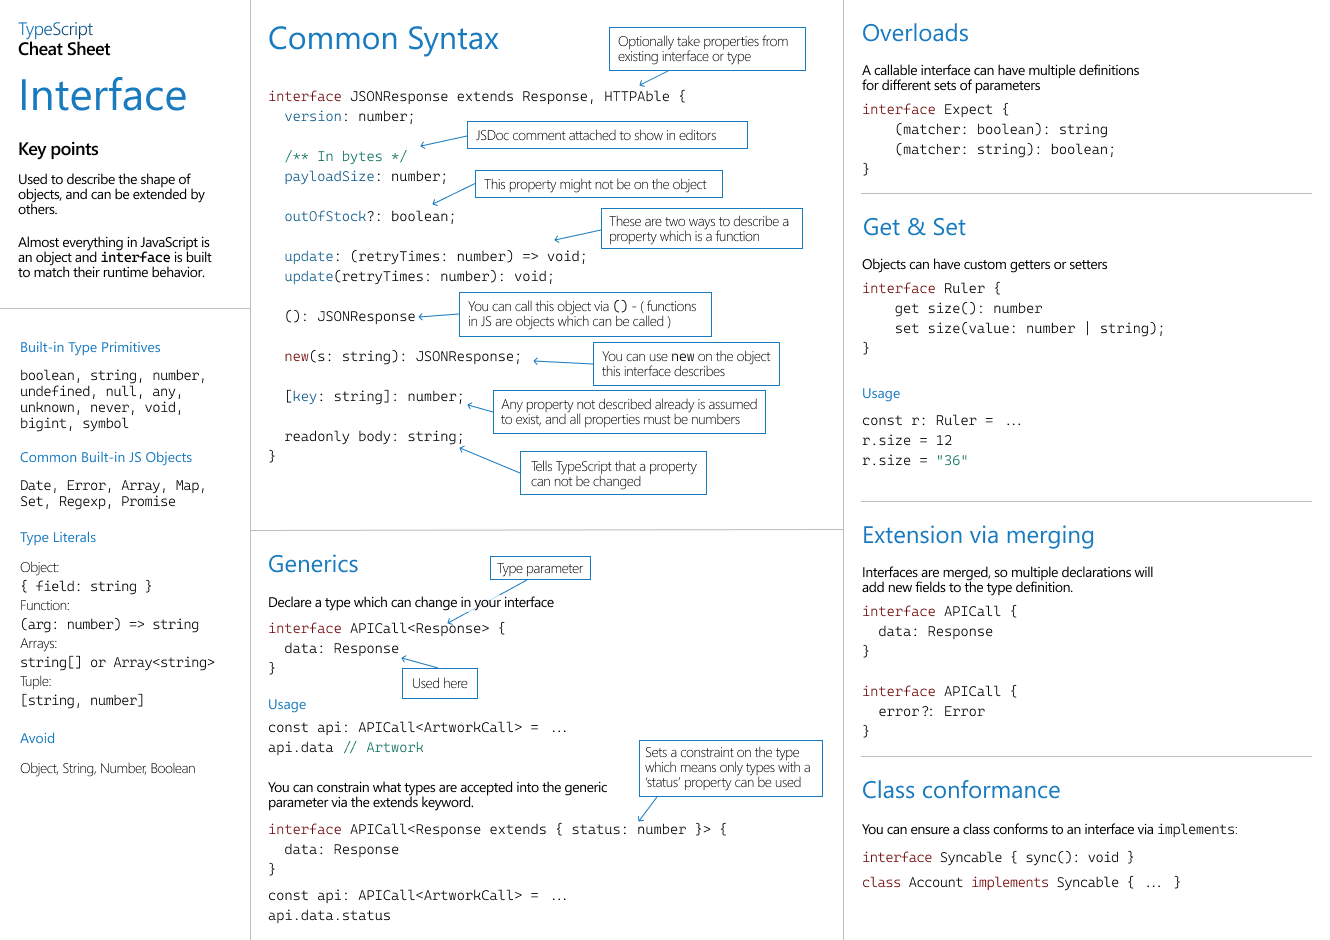
\includegraphics[width=0.8\textwidth]{TypeScriptInterfaces.png}
	\caption{Interfases}
\end{figure}

\begin{figure}[H]
	\center
	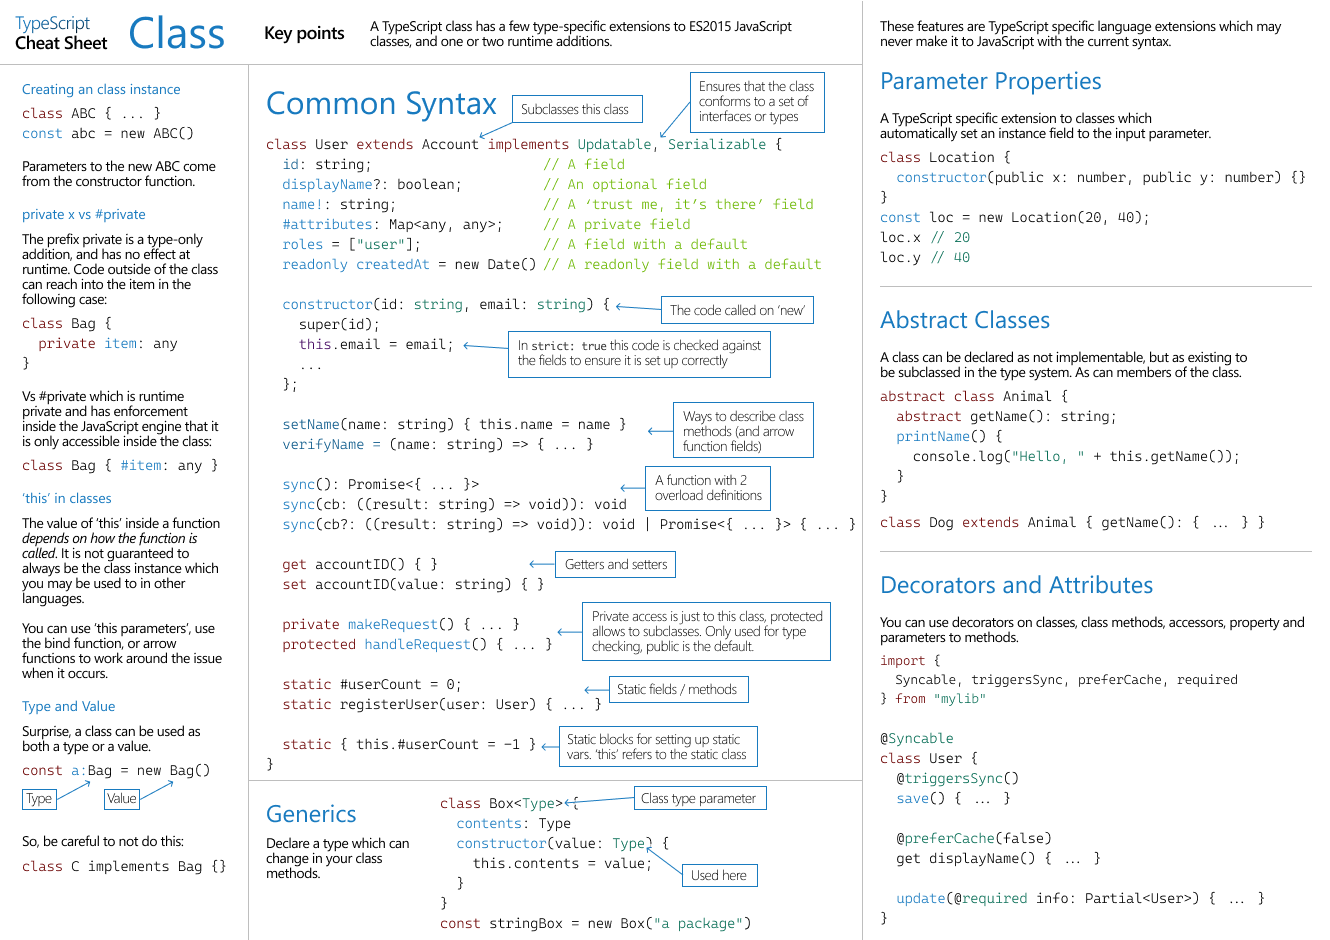
\includegraphics[width=0.8\textwidth]{TypeScriptClasses.png}
	\caption{Clases}
\end{figure}

\begin{figure}[H]
	\center
	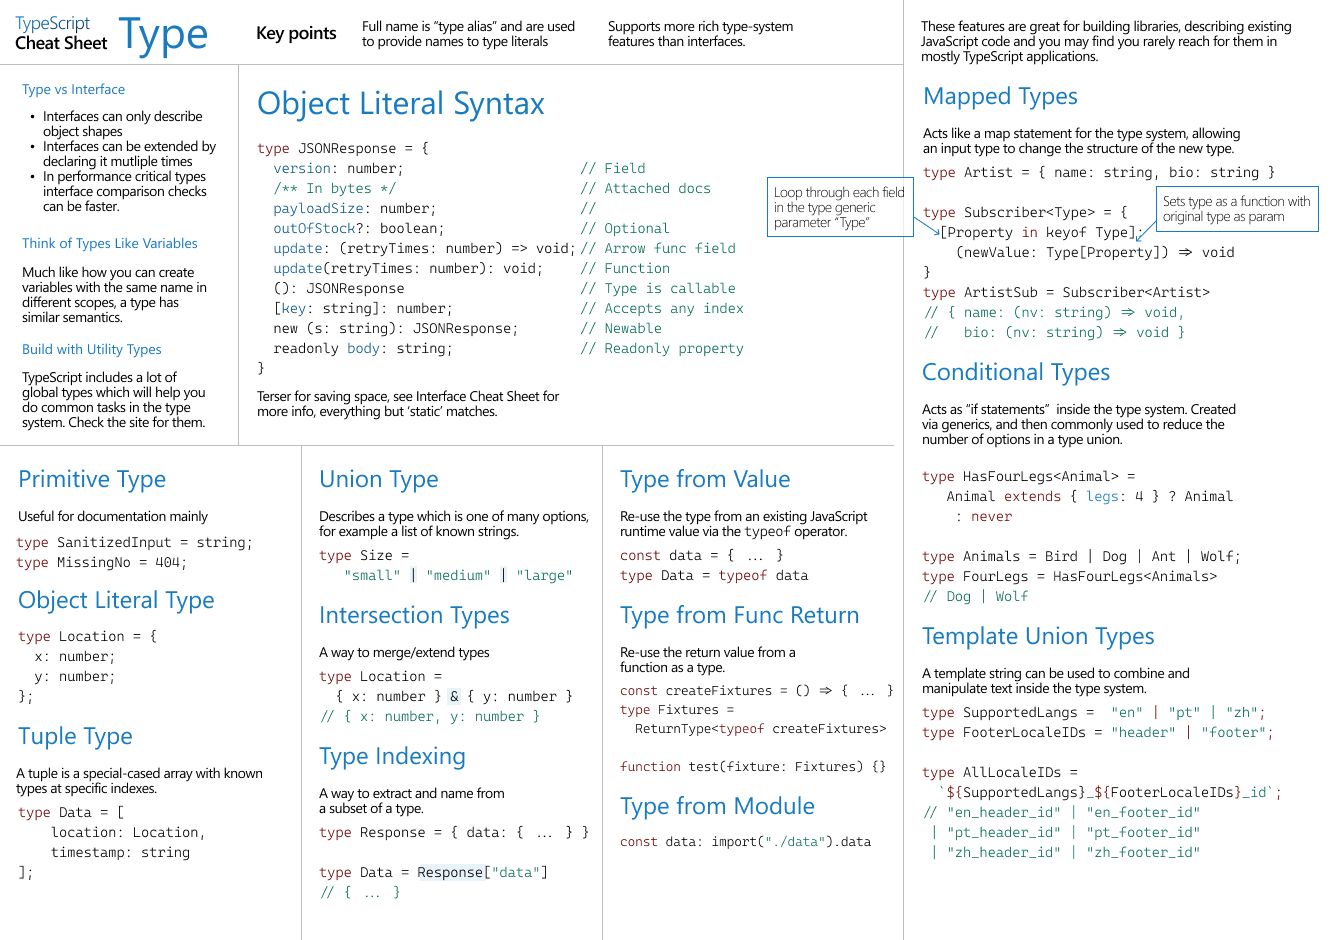
\includegraphics[width=0.8\textwidth]{TypeScriptTypes.png}
	\caption{Tipos}
\end{figure}

\url{https://www.typescriptlang.org/cheatsheets}

\subsection{Frameworks}

\cite{wiki}Un entorno de trabajo (del inglés framework), o marco de trabajo es un conjunto estandarizado
de conceptos, prácticas y criterios para enfocar un tipo de problemática particular que sirve como
referencia, para enfrentar y resolver nuevos problemas de índole similar.
En el desarrollo de software, un entorno de trabajo es una estructura conceptual y tecnológica
de asistencia definida, normalmente, con artefactos o módulos concretos de software, que puede
servir de base para la organización y desarrollo de software. Típicamente, puede incluir soporte
de programas, bibliotecas, y un lenguaje interpretado, entre otras herramientas, para así ayudar a
desarrollar y unir los diferentes componentes de un proyecto.
Representa una arquitectura de software que modela las relaciones generales de las entidades del
dominio, y provee una estructura y especial metodología de trabajo, la cual extiende o utiliza las
aplicaciones del dominio.

\begin{figure}[H]
	\center
	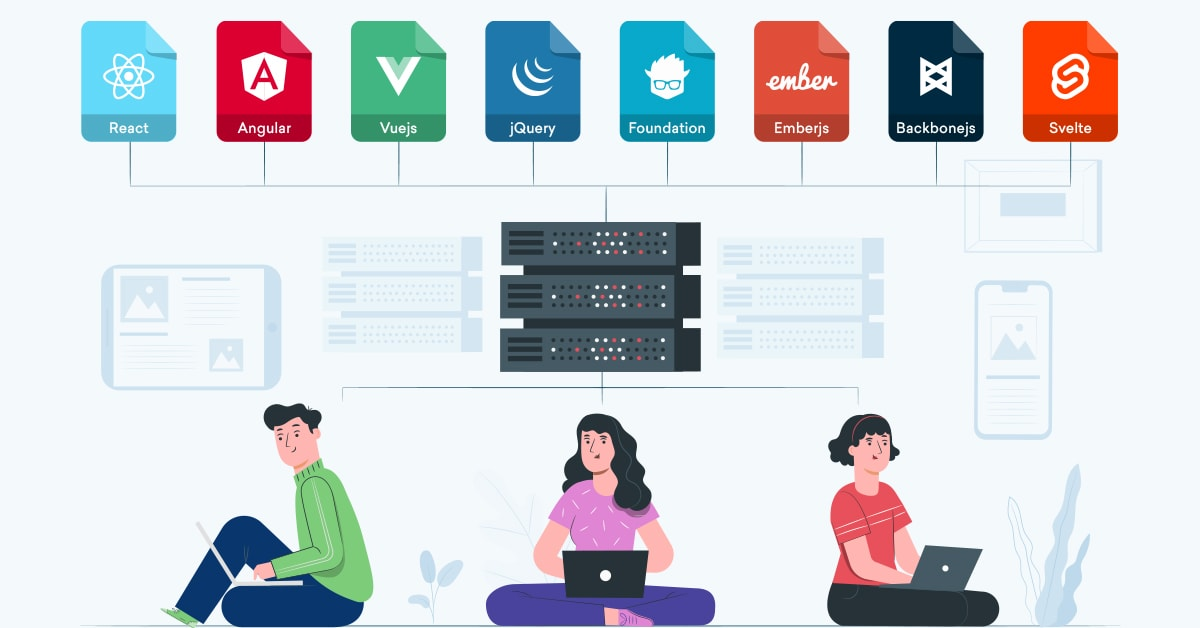
\includegraphics[width=0.7\textwidth]{frontend-frameworks-social.jpg}
	\caption{Algunos frameworks para frontend}
	\label{fig:super}
\end{figure}

\section{Estructura de datos}

\subsection{JSON}
\cite{json} JSON (Notación de objetos de JavaScript) es un formato ligero de intercambio de datos. Es fácil para los humanos leer y escribir. Es fácil para las máquinas analizar y generar. Se basa en un subconjunto del estándar de lenguaje de programación JavaScript ECMA-262 3ra edición - diciembre de 1999. JSON es un formato de texto que es completamente independiente del lenguaje pero utiliza convenciones que son familiares para los programadores de la familia de lenguajes C, incluidos C, C++, C#, Java, JavaScript, Perl, Python y muchos otros. Estas propiedades hacen de JSON un lenguaje de intercambio de datos ideal.

JSON se basa en dos estructuras:

\begin{itemize}
	\item Una colección de pares de nombre/valor. En varios idiomas, esto se realiza como un objeto , registro, estructura, diccionario, tabla hash, lista con clave o matriz asociativa.
	\item Una lista ordenada de valores. En la mayoría de los lenguajes, esto se realiza como una matriz , un vector, una lista o una secuencia.
\end{itemize}

Estas son estructuras de datos universales. Prácticamente todos los lenguajes de programación modernos los admiten de una forma u otra. Tiene sentido que un formato de datos que sea intercambiable con los lenguajes de programación también se base en estas estructuras.

En JSON, toman estas formas:

\begin{itemize}
	\item Un objeto es un conjunto desordenado de pares nombre/valor. Un objeto comienza con { llave izquierda y termina con } llave derecha . Cada nombre va seguido de : dos puntos y los pares de nombre/valor están separados por , coma .
	\begin{figure}[H]
		\center
		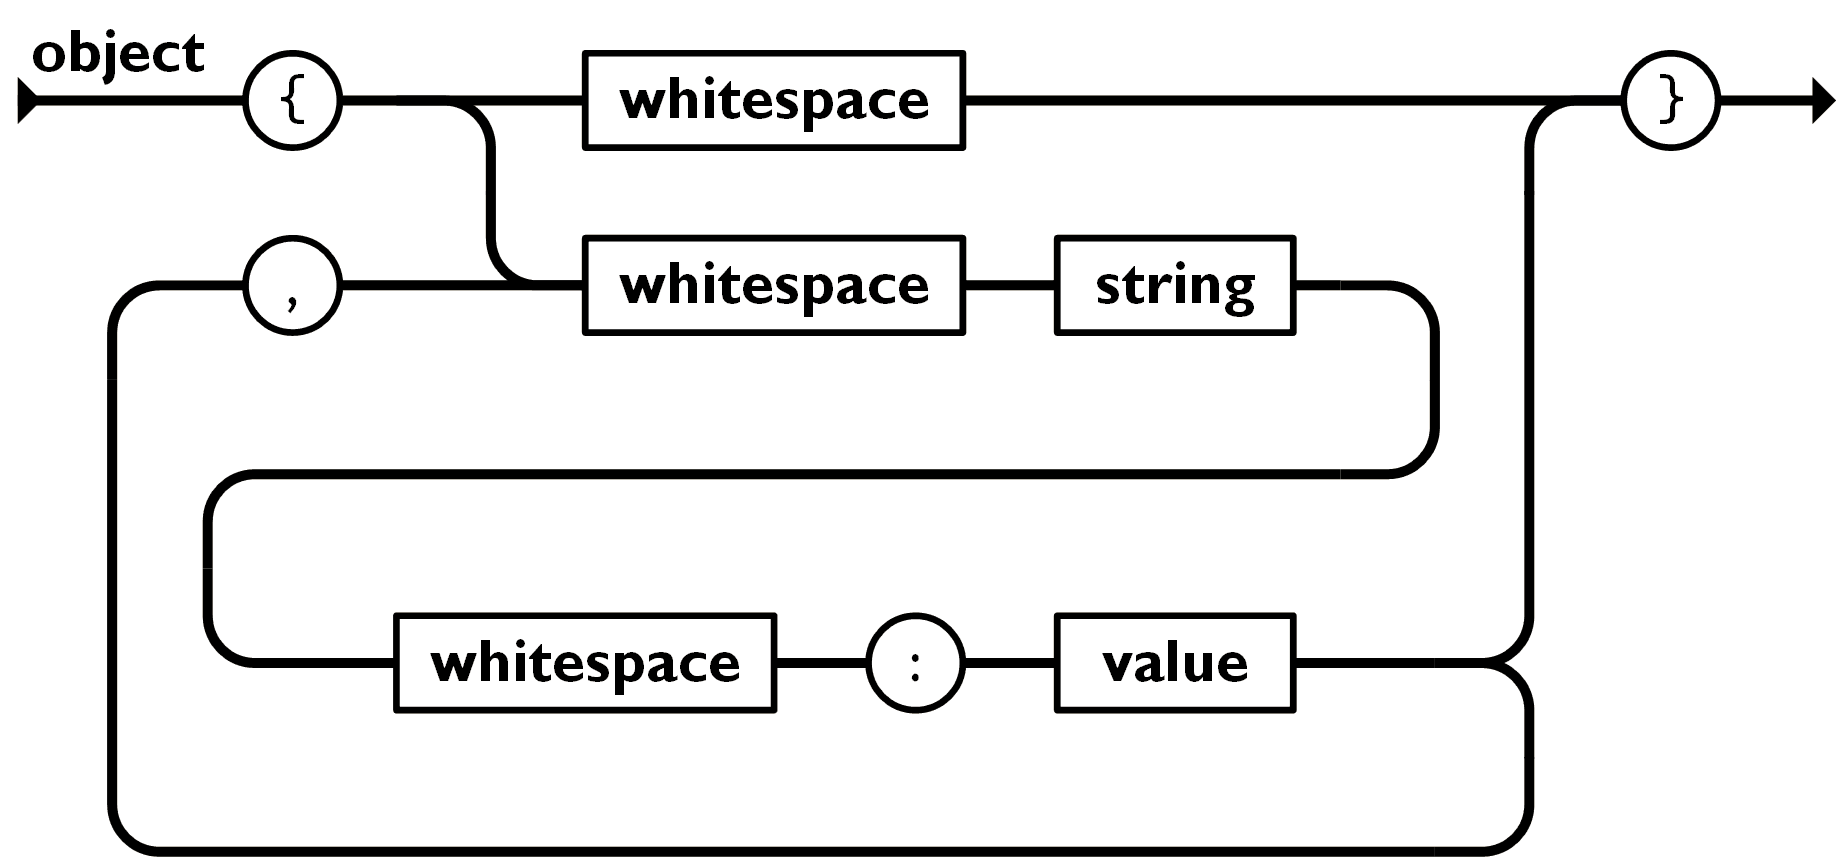
\includegraphics[width=0.5\textwidth]{object1.png}
		\caption{Clave valor}
	\end{figure}
	\item Una matriz es una colección ordenada de valores. Una matriz comienza con [ corchete izquierdo y termina con ] corchete derecho . Los valores están separados por comas .
	\begin{figure}[H]
		\center
		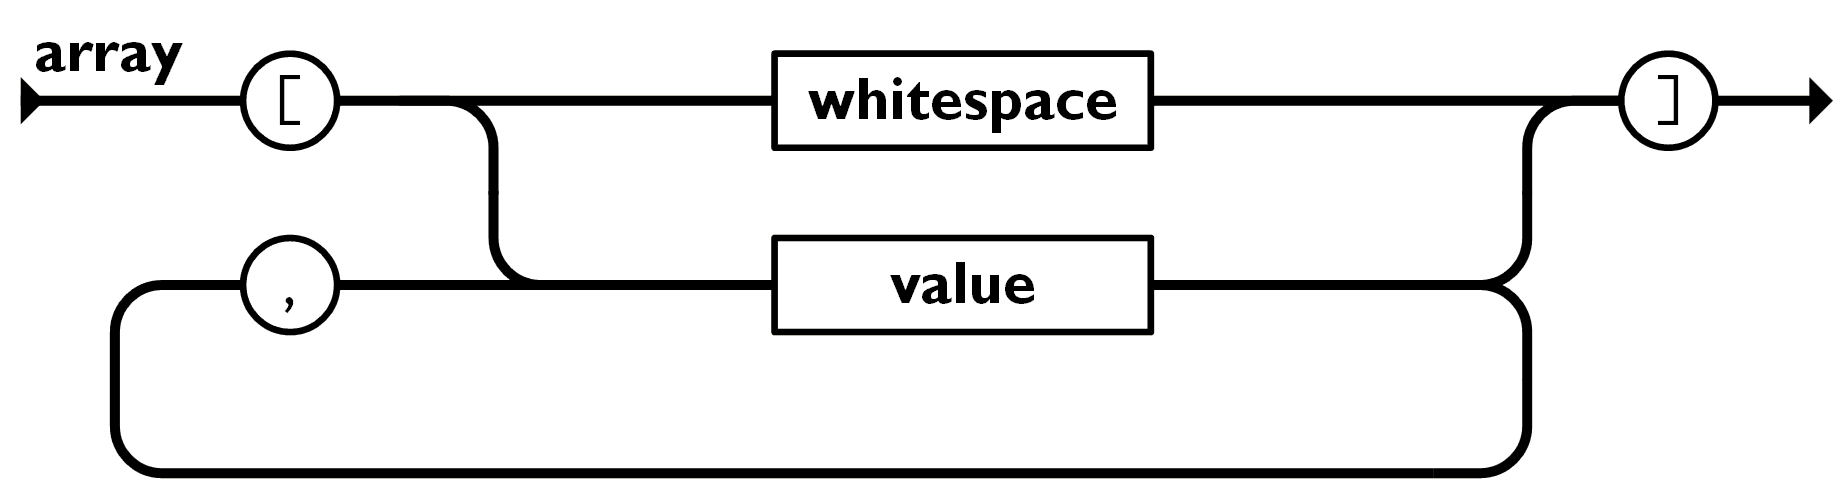
\includegraphics[width=0.5\textwidth]{array.png}
		\caption{Arreglo - Matriz}
	\end{figure}
\end{itemize}

Un valor puede ser una cadena entre comillas dobles, un número , verdadero , falso o nulo , un objeto o una matriz . Estas estructuras se pueden anidar.

	\begin{figure}[H]
	\center
	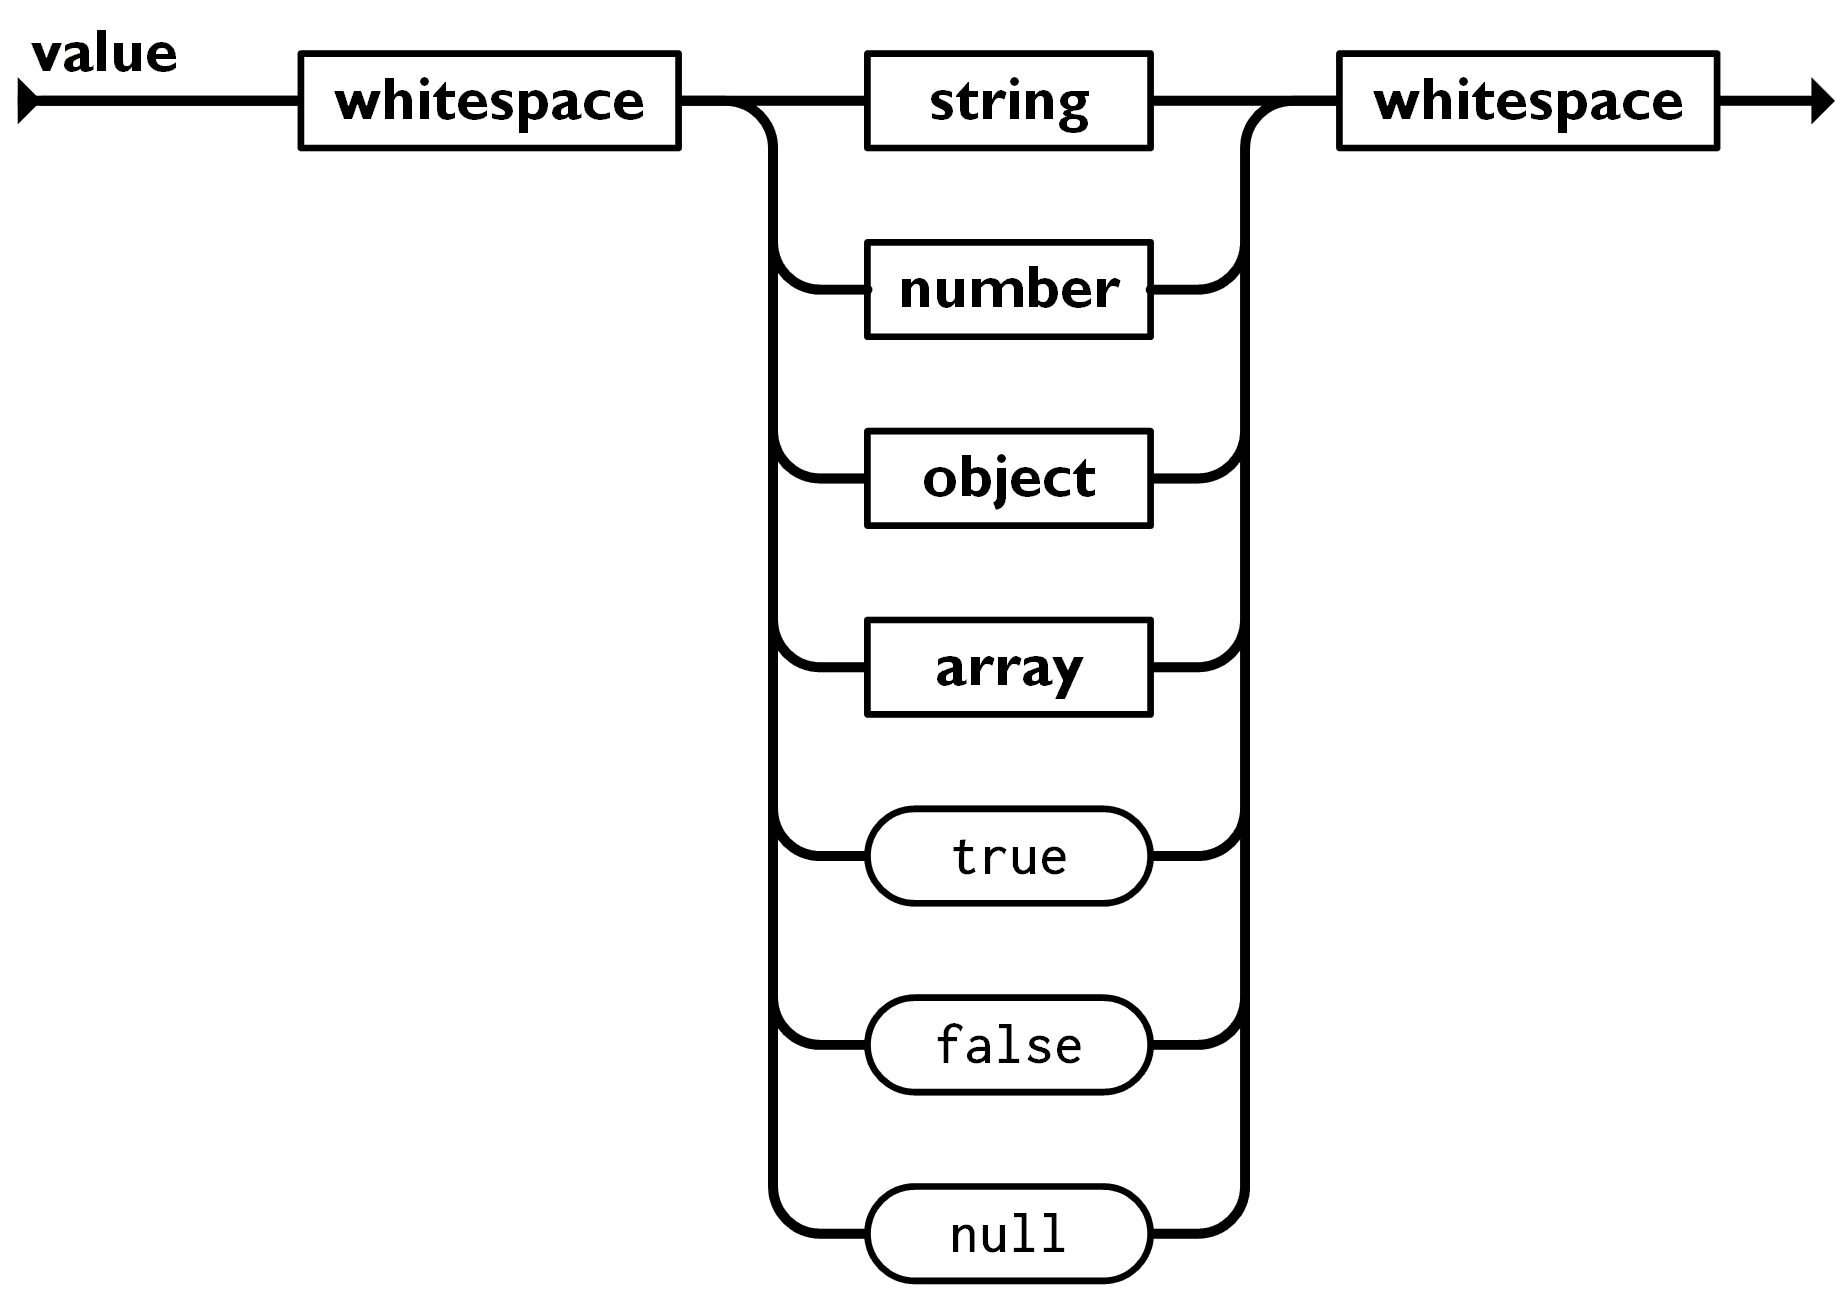
\includegraphics[width=0.5\textwidth]{value-json.png}
	\caption{Tipos de valores}
\end{figure}
\begin{remark}
Una cadena es una secuencia de cero o más caracteres Unicode, entre comillas dobles, usando escapes de barra invertida. Un carácter se representa como una sola cadena de caracteres. Una cadena es muy parecida a una cadena C o Java.
\end{remark}
\begin{remark}
Un número es muy parecido a un número de C o Java, excepto que no se utilizan los formatos octal y hexadecimal.
\end{remark}

\subsection{XML}

\cite{mdn} XML es un lenguaje de marcado similar a HTML. Significa Extensible Markup Language (Lenguaje de Marcado Extensible) y es una especificación de W3C como lenguaje de marcado de propósito general. Esto significa que, a diferencia de otros lenguajes de marcado, XML no está predefinido, por lo que debes definir tus propias etiquetas. El propósito principal del lenguaje es compartir datos a través de diferentes sistemas, como Internet.

Hay muchos lenguajes basados en XML; Algunos ejemplos son XHTML, MathML, SVG, XUL, XBL, RSS, y RDF. También puedes crear uno propio.

\subsubsection{XML "Correcto" (válido y bien formado)}

Para que un documento XML sea correcto, debe ser un documento bien formado, cumpliendo todas las reglas de sintaxis de XML, y válidas, acorde a las reglas de un lenguaje específico. Un ejemplo de un documento que no está bien formado es uno que tiene una etiqueta de apertura y no tiene una de cierre, ni se cierra en si misma.

En el ejemplo siguiente, vemos un documento en el que una etiqueta que no se cierra a si misma, no tiene etiqueta de cierre.

\begin{lstlisting}
<message>
	<warning>
		Hola, mundo
</message>
\end{lstlisting}

Ahora veamos una versión correcta del mismo documento:

\begin{lstlisting}
<message>
	<warning>
		Hola, mundo
	</warning>
</message>
\end{lstlisting}

Para ser válido, un documento XML necesita cumplir ciertas reglas de semántica que son generalmente definidas en un esquema XML o en una Definición de Tipo de Documento (en-US) (DTD). Un documento que contiene una etiqueta no definida es inválido. Por ejemplo, si nunca definimos la etiqueta <warning>, el documento anterior no sería válido.

\subsubsection{Arreglos en xml}

XML Array se ha definido como una matriz variable que agrupa los mismos elementos en la lista y contiene uno o más elementos secundarios. Los arreglos son una secuencia de elementos declarados con el mismo nombre.

La sintaxis general se muestra como:

\begin{lstlisting}
<?versión xml="1.0" codificación="utf-8"?>
<recursos>
	<item>recurso 1</item>
	<item>recurso 2</item>
	<item>recurso 3</item>		
</recursos>

\end{lstlisting}

\subsection{DTO}
\cite{mf}Un objeto que transporta datos entre procesos para reducir el número de llamadas a métodos.

Cuando trabaja con una interfaz remota, como Remote Facade (388), cada llamada es costosa. Como resultado, necesita reducir la cantidad de llamadas y eso significa que necesita transferir más datos con cada llamada. Una forma de hacer esto es usar muchos parámetros. Sin embargo, esto a menudo es complicado de programar; de hecho, a menudo es imposible con lenguajes como Java que devuelven un solo valor.

La solución es crear un objeto de transferencia de datos que pueda contener todos los datos de la llamada. Debe ser serializable para atravesar la conexión. Por lo general, se usa un ensamblador en el lado del servidor para transferir datos entre el DTO y cualquier objeto de dominio.

Aunque la razón principal para usar un objeto de transferencia de datos es agrupar lo que serían múltiples llamadas remotas en una sola llamada, vale la pena mencionar que otra ventaja es encapsular el mecanismo de serialización para transferir datos por cable. Al encapsular la serialización de esta manera, los DTO mantienen esta lógica fuera del resto del código y también brindan un punto claro para cambiar la serialización si lo desea.

\begin{figure}[H]
	\center
	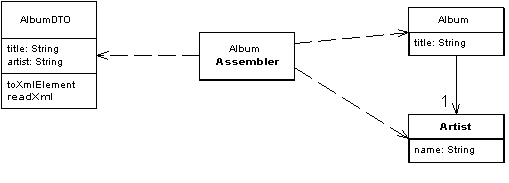
\includegraphics[width=1\textwidth]{dtoSketch.png}
	\caption{Ejemplo de un DTO}
\end{figure}

\section{Localización e Internacionalización}

\cite{w3}¿Qué significan los términos "internacionalización" y "localización" y cómo se relacionan?

Ofrecemos aquí algunas descripciones generales, de alto nivel, que reflejan el modo en que tendemos a utilizar estos términos en el sitio del W3C dedicado a la internacionalización.

\subsection{Localización}

Se entiende por localización la adaptación de un producto, una aplicación o el contenido de un documento con el fin de adecuarlos a las necesidades (lingüísticas, culturales u otras) de un mercado destinatario concreto (una "localidad" o "local" [locale]).

\begin{remark}
	La palabra localización a veces se escribe "l10n", donde 10 es la cantidad de letras entre la ele y la ene.
\end{remark}


Aunque se la considera a menudo sinónimo de traducción de la interfaz de usuario y de la documentación, la localización suele ser un asunto considerablemente más complejo, que puede implicar la adaptación del contenido en relación con:

\begin{enumerate}
	\item formatos numéricos, de fecha y de hora;
	\item uso de símbolos de moneda;
	\item uso del teclado;
	\item algoritmos de comparación y ordenamiento;
	\item símbolos, iconos y colores;
	\item texto y gráficos que contengan referencias a objetos, acciones o ideas que, en una cultura dada, puedan ser objeto de mala interpretación o considerados ofensivos;
	\item diferentes exigencias legales;
	\item y muchas otras cuestiones.
\end{enumerate}

La localización puede requerir incluso una reelaboración exhaustiva de la lógica, el diseño visual o la presentación, si la forma de hacer negocios (por ejemplo, las normas contables) o el paradigma aceptado de aprendizaje (por ejemplo, énfasis en el individuo o en el grupo) en la localidad de destino difieren mucho en relación con la cultura originaria.

\subsection{Internacionalización}

Existen diferentes definiciones para la palabra internacionalización. La que damos aquí es una definición operativa de alto nivel para usar con los materiales de la Actividad de internacionalización del W3C. Algunas personas utilizan otros términos para referirse al mismo concepto, por ejemplo, "globalización".

La internacionalización es el diseño y desarrollo de un producto, una aplicación o el contenido de un documento de modo tal que permita una fácil localización con destino a audiencias de diferentes culturas, regiones o idiomas.
\begin{remark}
	La palabra internacionalización a veces se escribe "i18n", donde 18 es la cantidad de letras entre la i y la ene.
\end{remark}

La internacionalización generalmente implica:

\begin{enumerate}
	\item Un modo de diseño y desarrollo que elimine obstáculos a la localización o la distribución internacional. Esto incluye cuestiones tales como (entre otras) usar Unicode o asegurar, allí donde corresponda, un correcto tratamiento de las codificaciones de caracteres anticuadas; controlar la concatenación de cadenas; o evitar que la programación dependa de valores de cadenas pertenecientes a la interfaz de usuario.
	\item Habilitar características que tal vez no sean usadas hasta el momento de la localización. Por ejemplo, añadir en la DTD etiquetas para habilitar el texto bidireccional o la identificación de idiomas. O hacer la CSS compatible con texto vertical u otras características tipográficas ajenas al alfabeto latino.
	\item Preparar el código para hacer frente a las preferencias locales, regionales, lingüísticas o culturales. Por lo general, esto supone incorporar características y datos de localización predefinidos a partir de bibliotecas existentes o de las preferencias del usuario. Algunos ejemplos son: formatos de fecha y hora, calendarios locales, formatos y sistemas de números, ordenamiento y presentación de listas, uso de nombres personales y formas de tratamiento, etc.
	\item Separar del código o contenido fuente los elementos localizables, de modo que puedan cargarse o seleccionarse alternativas localizadas según determinen las preferencias internacionales del usuario.
\end{enumerate}

Obsérvese que esta lista no incluye necesariamente la localización del contenido, la aplicación o el producto hacia otro idioma; se trata más bien de prácticas de diseño y desarrollo que facilitan esa migración en el futuro, pero que también pueden tener una utilidad considerable aunque la localización jamás se produzca.

La internacionalización influye considerablemente en la facilidad de localización del producto. Obviamente, resulta mucho más difícil y demanda mucho más tiempo adaptar retrospectivamente un producto centrado en un idioma y cultura particulares que diseñarlo desde un primer momento con la intención de presentarlo mundialmente. (Piénsese en el Y2K y todo lo que demandó tratar de "deshacer" la opción por campos de fecha de dos caracteres, basada en el supuesto de que se interpretarían siempre como "19xx").

De modo que, en condiciones ideales, la internacionalización se da como un paso fundamental en el proceso de diseño y desarrollo, más que como un agregado posterior que, a menudo, puede implicar un difícil y costoso proceso de reingeniería.